\documentclass[12pt]{article}

% Packages
\usepackage{float}
\usepackage{amsmath}
\usepackage{amsfonts}
\usepackage{subcaption}
\usepackage{graphicx}
\usepackage{listingsutf8}
\usepackage[utf8]{inputenc}
\usepackage{xcolor}
\usepackage[a4paper, total={16cm, 23.7cm}]{geometry}
\usepackage[colorlinks=true,urlcolor=blue]{hyperref}
\usepackage{color}

% Compiler/IDE directives
% !TeX spellcheck = en_US

% General
\fontfamily{phv}
\captionsetup{width=0.8\textwidth}

% Graphicx
\graphicspath{ {./images/} }
 
% Listings
\definecolor{codegreen}{rgb}{0,0.6,0}
\definecolor{codegray}{rgb}{0.5,0.5,0.5}
\definecolor{codepurple}{rgb}{0.58,0,0.82}
\definecolor{backcolour}{rgb}{0.95,0.95,0.92} 
\lstdefinestyle{mystyle}{
    backgroundcolor=\color{backcolour},   
    commentstyle=\color{codegreen},
    keywordstyle=\color{magenta},
    numberstyle=\tiny\color{codegray},
    stringstyle=\color{codepurple},
    basicstyle=\fontsize{7}{9}\selectfont\ttfamily,
    breakatwhitespace=false,         
    breaklines=true,                 
    captionpos=b,                    
    keepspaces=true,                 
    numbers=left,                    
    numbersep=5pt,                  
    showspaces=false,                
    showstringspaces=false,
    showtabs=false,                  
    tabsize=2
}
\lstset{style=mystyle}

% Geometry
\DeclareMathSizes{12}{13}{10}{8}
\setlength\parindent{0.7cm}

% Helper commands
\newcommand*\diff{\mathop{}\!\mathrm{d}}
\newcommand*\Diff[1]{\mathop{}\!\mathrm{d^#1}}
\newcommand\tab[1][.7cm]{\hspace*{#1}}
\renewcommand{\refname}{}
\newcommand{\code}[1]{\texttt{#1}}


%----------------------------------------------------------------------------
% THE DOCUMENT
%----------------------------------------------------------------------------
\begin{document}


%----------------------------------------------------------------------------
% TITLE
%----------------------------------------------------------------------------
\begin{center}
	\Huge Performance optimization of the online data processing software for a high-energy physics experiment\\
	\Large Thesis report\\
	\vspace{1pc}
	\huge Péter Kardos \\
	\large 2018-2019
\end{center}


%----------------------------------------------------------------------------
% === ABSTRACT ===
%----------------------------------------------------------------------------
\section*{Abstract}

The LHCb experiment probes into the differences between matter and anti-matter by examining particle collisions. Like any modern high energy physics experiment, LHCb relies on a complex hardware and software infrastructure to collect and analyze the data generated from particle collisions. To filter out unimportant data before writing it to permanent storage, particle collision events have to be processed in real-time which requires a lot of computing power.
This thesis focuses on performance optimizations of several parts of the real-time data processing software: i) one of the particle path reconstruction steps; ii) the particle path refining step; iii) the data structures used by the real-time reconstruction algorithms. The thesis investigates and employs techniques such as vectorization, cache-friendly memory structures, microarchitecture analysis, and memory allocation optimizations.
The resulting performance-optimized code uses today's many-core, data-parallel, superscalar processors to their full potential in order to meet the performance demands of the experiment. The thesis results show that the reconstruction step got 3 times faster, the refinement step got 2 times faster and the changes to the data model allowed vectorization of most reconstruction algorithms.


%----------------------------------------------------------------------------
% === TABLE OF CONTENTS, FIGURES, TABLES ===
%----------------------------------------------------------------------------

\newpage
{
	\small
	\hypersetup{linkcolor=black}
	\tableofcontents
}

{
	\small
	\hypersetup{linkcolor=black}
	\listoffigures
}

{
	\small
	\hypersetup{linkcolor=black}
	\listoftables
}

{
	\small
	\renewcommand\lstlistlistingname{Code Listings}
	\hypersetup{linkcolor=black}
	\lstlistoflistings
}

%----------------------------------------------------------------------------
% === GLOSSARY ===
%----------------------------------------------------------------------------


\section*{Abbreviations}

\begin{itemize}
	\item ALICE: A Large Ion Collider Experiment
	\item AMD: Advanced Micro Devices
	\item AOS: Array Of Structures
	\item ATLAS: A Toroidal LHC ApparatuS
	\item AVX: Advanced Vector eXtensions
	\item BMI: Bit Manipulation Instructions
	\item CCD: Charge Coupled Device
	\item CERN:  Conseil Européen pour la Recherche Nucléaire
	\item CMOV: Conditional MOVe (x86 CPU instruction)
	\item CMS: Compact Muon Solenoid
	\item CPU: Central Processing Unit
	\item DRAM: Dynamic Random Access Memory
	\item FMA: Fused Multiply-Add
	\item FP: Floating Point
	\item FPGA: Field Programmable Gate Array
	\item FT: (Scintillating) Fiber Tracker
	\item IPC: Instructions Per Cycle
	\item ISA: Instruction Set Architecture
	\item L1, L2, L3: Level 1, 2, 3 CPU caches
	\item LHC: Large Hadron Collider
	\item LHCb: Large Hadron Collider beauty
	\item OS: Operating System
	\item PCB: Printed Circuit Board
	\item POD: Plain Old Data
	\item RICH: Ring Imaging CHerenkov (detector)
	\item SIMD: Single Instruction Multiple Data
	\item SOA: Structure Of Arrays
	\item SP: Space Partitioning (not used in literature)
	\item SSE: Streaming SIMD Extensions 
	\item TT: Trigger Tracker
	\item UT: Upstream Tracker
	\item VELO: VErtex LOcator
\end{itemize}


\section*{Definitions}

\begin{itemize}
	\item Algorithm: building blocks of the \textit{event reconstruction} software of LHCb.
	\item Benchmarking: analyzing the performance (execution time) of a piece of software.
	\item Cache \& data layout optimization: transform code taking into consideration the internal behaviour of the CPUs' multi-level cache architecture and future goals such as vectorization.
	\item Event: the collision of two LHC particle beam bunches inside the LHCb detector.
	\item Hit: the unique identifier of a single pixel or fiber of a subdetector that was hit by a particle in an event.
	\item Hotspots: the few small, independent parts of the code that consume the vast majority of CPU execution time.
	\item Momentum: as in momentum of a particle, $\Vec{p}=m\Vec{v}$.
	\item Multi-threading: using multiple operating system threads to do computation work in parallel.
	\item Node: as in part of a \textit{server farm} or supercomputer; a normal server computer, running its own operating system on its own hardware resources.
	\item Processing events/event reconstruction: recreate the \textit{tracks} from the set of \textit{hits} provided by the subdetectors.
	\item Server farm: an interconnected network of \code{nodes}, where the node run independently but can communicate with each other.
	\item Streamline (the code): remove unnecessary parts, reduce complexity, optimize instructions.
	\item Superscalar architecture: modern CPU architectures whose implementation does not conform to the linear, scalar execution model of CPUs. (Their programming interface does, however.) Features include multiple execution units and out-of-order execution.
	\item Track: LHCb software's representation of the path of a particle, a selection of \textit{hits}.
	\item Type of tracks: LHCb \textit{tracks} are categorized based on the subdetectors they have interacted with.
	\item Vectorization: the act of transforming code to use data-parallel (SIMD) CPU instruction sets without changing the behaviour of the code.
\end{itemize}


%----------------------------------------------------------------------------
% === Introduction ===
%----------------------------------------------------------------------------
\newpage
\section{Introduction}\label{sec_intro}

\subsection{Particle accelerators}\label{sec_part_accel_intro}

\subsubsection{Idea and purpose}\label{sec_part_accel_idea}

CERN (European Organization for Nuclear Research) is an international high energy experimental physics research organization situated near Geneva, on the Franco-Swiss border. CERN's research is based around its infrastructure of several particle accelerators, including the world's largest particle accelerator. Physics research data is obtained from colliding the accelerated particles, and is meant to probe the fundamental laws of the universe. In general, research is organized into \textit{experiments}, each of which examines a particular physics phenomenon. Experiments are using the particle accelerator infrastructure, but have their own devices for the experiment's specific goals.
\cite{cern_about}

\vspace{1pc}\noindent
Particle accelerators accelerate charged particles to high velocities using magnetic and electric fields, then the particles are made to collide with a stationary target or other particles going in the opposite direction. Einstein's famous formula, $E=mc^2$ describes how energy can be converted into matter and vice versa. In a collision, the mass of the colliding particles and their kinetic energy gets converted into new particles in a quantum process. The new particles also have some kinetic energy, thus fly away from the collision point. Thanks to the high energy of the collision, heavy particles that are otherwise extremely rare also get created and scientists can examine their properties in a controlled environment.

\subsubsection{Theory of operation}\label{sec_part_accel_theory}

\begin{figure}[H]
	\begin{center}
		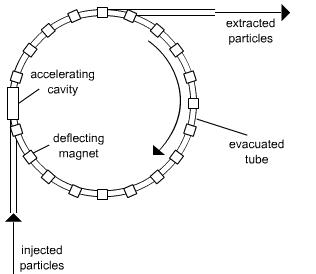
\includegraphics[width=0.5\textwidth]{particle_accelerator_schematic}
	\end{center}
	\caption[Circular particle accelerator structure]{Simplified schematic of a circular particle accelerator with the crucial functional parts labelled. \cite{accelerator_image_src_1}}
	\label{fig_part_accel_schematic}
\end{figure}

Particle accelerators can be circular or linear. Figure \ref{fig_part_accel_schematic} depicts a circular accelerator, which consists of the following parts:
\begin{itemize}
	\item Evacuated tube (beam pipe): a closed, circular tube in which the particles can travel. To avoid the particles colliding with air particles, it is strictly under vacuum.
	\item Particle source: injects the particles into the beam pipe. For proton accelerators, a bottle of hydrogen serves as the source. The hydrogen atoms are ionized, and then linearly accelerated by an electric field before entering the circular beam pipe.
	\item Accelerating cavity: uses oscillating electromagnetic fields which are timed to provide a push to the charged particles via electric force, accelerating them.
	\item Deflecting magnet: using the Lorentz-force, a strong magnetic field steers the particles inwards to the center of the circle, keeping it on the circular trajectory.
	\item Extraction pipe: once the particles are fast enough, they are extracted from the circular beam pipe to collide with a stationary target.
\end{itemize}

The particle is at first injected to the beam pipe at a low energy. Thanks to the deflecting magnets, it keeps revolving in the beam pipe for thousand of revolutions. Each turn, particles get boosted by the accelerating cavities as they pass by, increasing their energy. When particles reach their maximum energy, which is determined by the strength of the steering magnets and the circumference of the accelerator, they are extracted from the beam pipe to collide with a stationary target.

It is not individual particles that revolve around the accelerator, rather, it's a swarm of millions of particles distributed throughout the entire circle. The distribution of the particles is not uniform. The particles group into \textit{bunches} which are equally spaced along the circle.

In addition to deflecting magnets, accelerators also employ \textit{focusing magnets}. Their purpose is to squeeze the bunches in the directions perpendicular to the particles' velocity, resulting in the beam having a smaller cross-section. Without focusing magnets, the bunches would slowly disintegrate and the particles would hit the wall of the beam pipe.

Linear accelerators contain the same functional elements as circular ones, but they don't need deflecting magnets since the particles travel in a straight path.


\subsubsection{Particle colliders}\label{sec_part_collider}

Colliders have two beams right next to each-other, but the particles are revolving in the opposite directions. This is achieved either by having two beam pipes (as in the LHC) or the two beams sharing the same beam pipe (like in LEP). At some specific points, the beams are crossed and the bunches collide with each other. It is important to mention that even though a bunch contains about $1.2\cdot 10^11$ protons\cite{lhc_facts_and_figures} in case of the LHC, the protons are so small thus the bunch is so sparse that only about 40 proton-proton collisions occur (in case of the ATLAS experiment) per bunch collision.


\subsection{The accelerator complex}\label{sec_accel_complex}

\begin{figure}[H]
	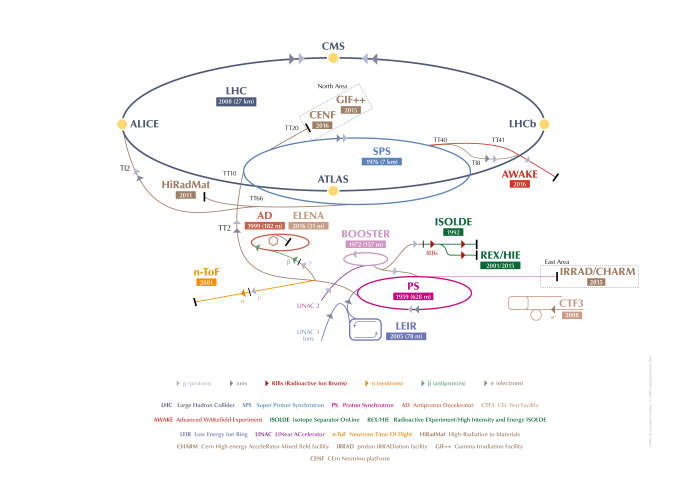
\includegraphics[width=\textwidth]{accelerator_complex}
	\caption[CERN accelerator complex]{Schematic view of CERN's particle accelerators and experiments. LHC is shown on top by the largest circle. The four main experiments, CMS, ALICE, ATLAS and LHCb are marked with yellow dots along the LHC's circle. \cite{cern_document_server}.}
	\label{fig_accel_complex}
\end{figure}

As seen on \ref{fig_accel_complex}, CERN hosts a complex system of particle accelerators\cite{cern_accel_complex}.
The LHC, shown in dark blue, is the subject of this thesis project. The LHC is a particle collider, the energy of individual particles reaches about 7 TeVs at maximum. The particle collisions occur at 4 points, marked CMS, ALICE, LHCb and ATLAS. At these points, particle detectors are installed to analyze the collisions. Detectors track the path of the particles and measure their properties such as momentum, charge and mass. Using these properties, particles can be identified. The raw data provided by the detectors is processed by software.


\subsection{LHCb experiment's detector}\label{sec_lhcb_detector}	

\subsubsection{Construction of the detector}\label{sec_lhcb_det_constr}

\begin{figure}[H]
	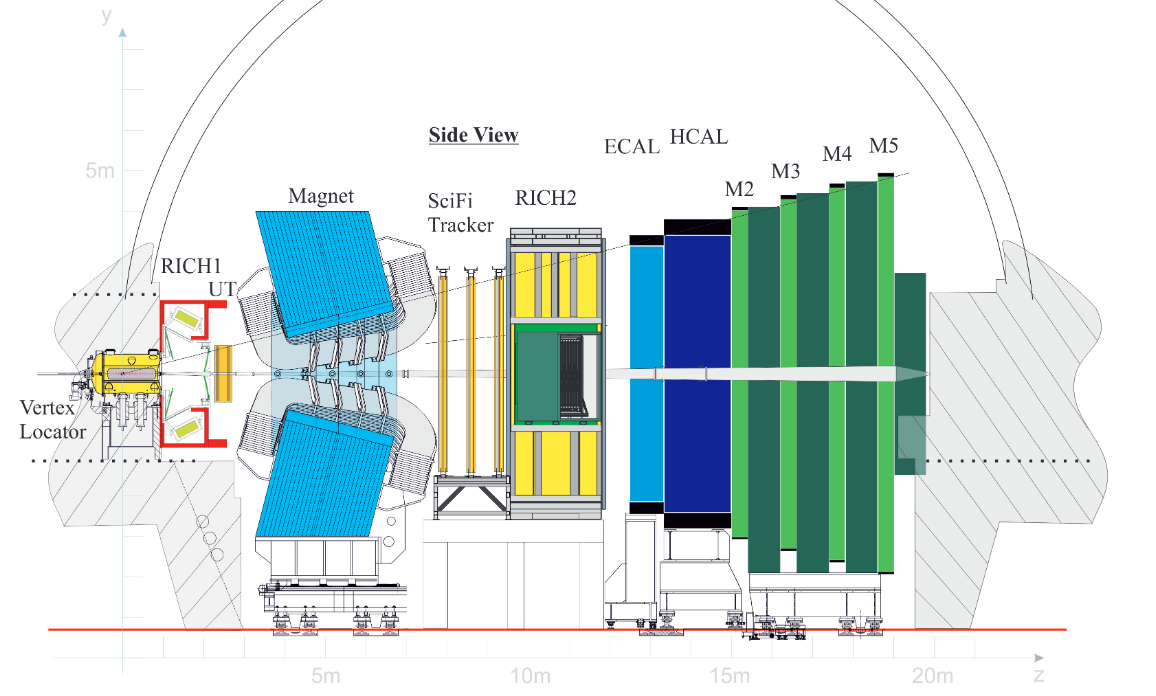
\includegraphics[width=\textwidth]{lhcb_geometry_upgrade}
	\caption[LHCB detector side view]{Side view of the LHCb detector. \cite{tracker_tdr}}
	\label{fig_lhcb_geometry}
\end{figure}

Figure \ref{fig_lhcb_geometry} shows the LHCb detector from the side, the two beams of the LHC go in the horizontal direction on the drawing, through the middle of the detector. The detector is both vertically and horizontally symmetric to the beampipe.

As seen on the labels, the detector consists of multiple layers of sub-detectors. Each layer has a hole in the center to let the beam pipes through. The two particle beams cross each other inside the Vertex Locator (VELO, at the right in yellow). As opposed to most other detectors, this one only analyzes the products of the collision in a narrow cone away from the VELO. The parts from RICH to M5 could be mirrored around the VELO to have two cones that touch each other by the tip, however it is not done for financial reasons.

The goal of the LHCb detector is the same as for all other detectors: reconstruct the paths and types of the particles. Even though full reconstruction uses all sub-detectors, we are only interested in partial reconstruction that can be done in real-time. This only involves the VELO, the UT (in orange, right of VELO) and the FT (SciFi Tracker, in the middle in orange).


\subsubsection{Coordinate system}\label{sec_coordinate_system}

The LHCb detector's coordinate system is used for calculations. The Z axis points down the beamline, the Y axis points upwards and the X axis to the left (as seen when looking down the Z axis). The LHC itself and civil engineering works use different labelling or alignment for the their coordinate axes.

\begin{figure}[H]
	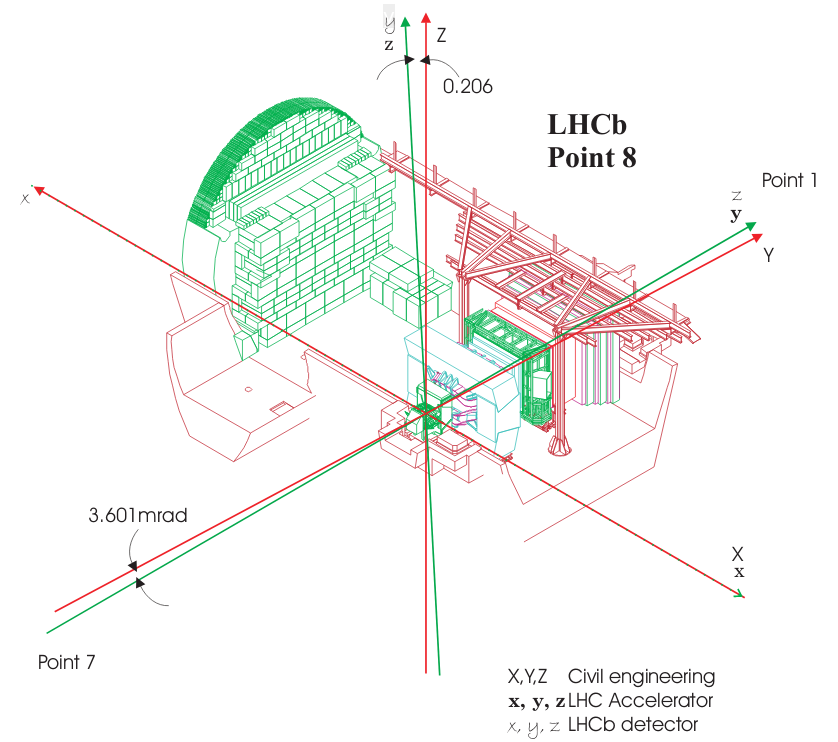
\includegraphics[width=\textwidth]{intro_lhcb_coordinate_systems}
	\caption[LHCb coordinate systems]{The different coordinate systems used in the LHCb cavern. \cite{lhcb_coordinate_systems}}
	\label{fig_lhcb_coordinate_systems}
\end{figure}


\subsubsection{Operating principles}\label{sec_lhcb_det_theory}

\begin{figure}[H]
	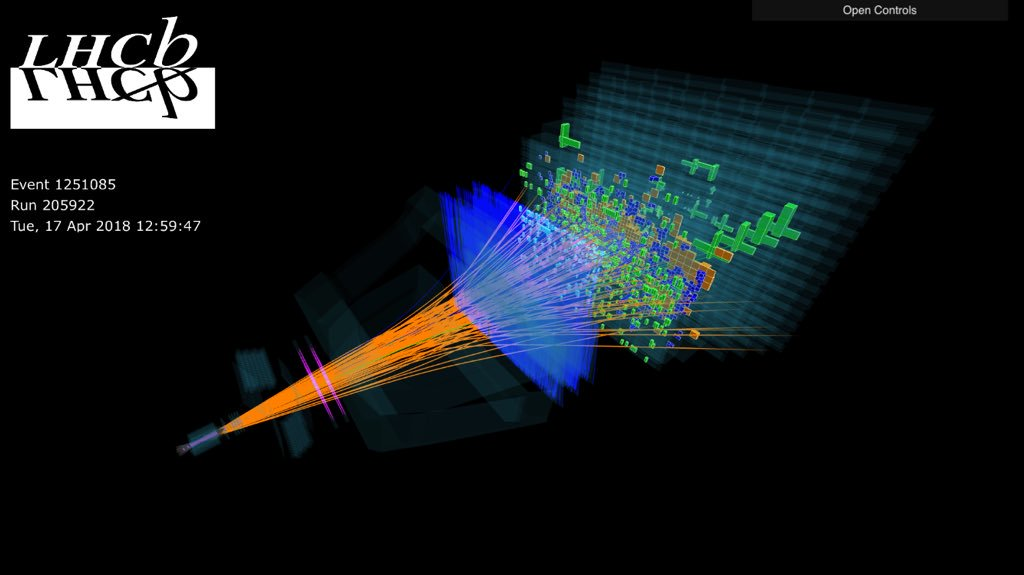
\includegraphics[width=\textwidth]{lbevent_collision_example}
	\caption[A particle collision event in LHCb]{Particles created in a real collision and their interaction with the detector. \cite{lb_event_display}}
	\label{fig_lhcb_lbevent_collision}
\end{figure}


Figure \ref{fig_lhcb_lbevent_collision} shows one particle collision event's results. The particles that were born in the collision are shown by the orange lines. The three aforementioned detectors, the VELO, UT and FT, can be identified by the origin of the orange particles, the pink cloud of lines and the bright blue cloud lines, respectively. The green and yellow cubic illustrations on the far-end of the detector belong to other sub-detectors, and are out of the scope of this paper.

The VELO is a small detector, it measures less than a meter in length. It is a silicon pixel detector, which looks much like a modern CCD camera: a rectangular array of pixels which detect light (or in this case, particles) that hit it. The difference is that particle detectors don't absorb the particle, rather, it passes through largely undisturbed. Additionally, the VELO consists of 26 such CCD-like rectangles, instead of just one.

\begin{figure}[H]
	\begin{center}
		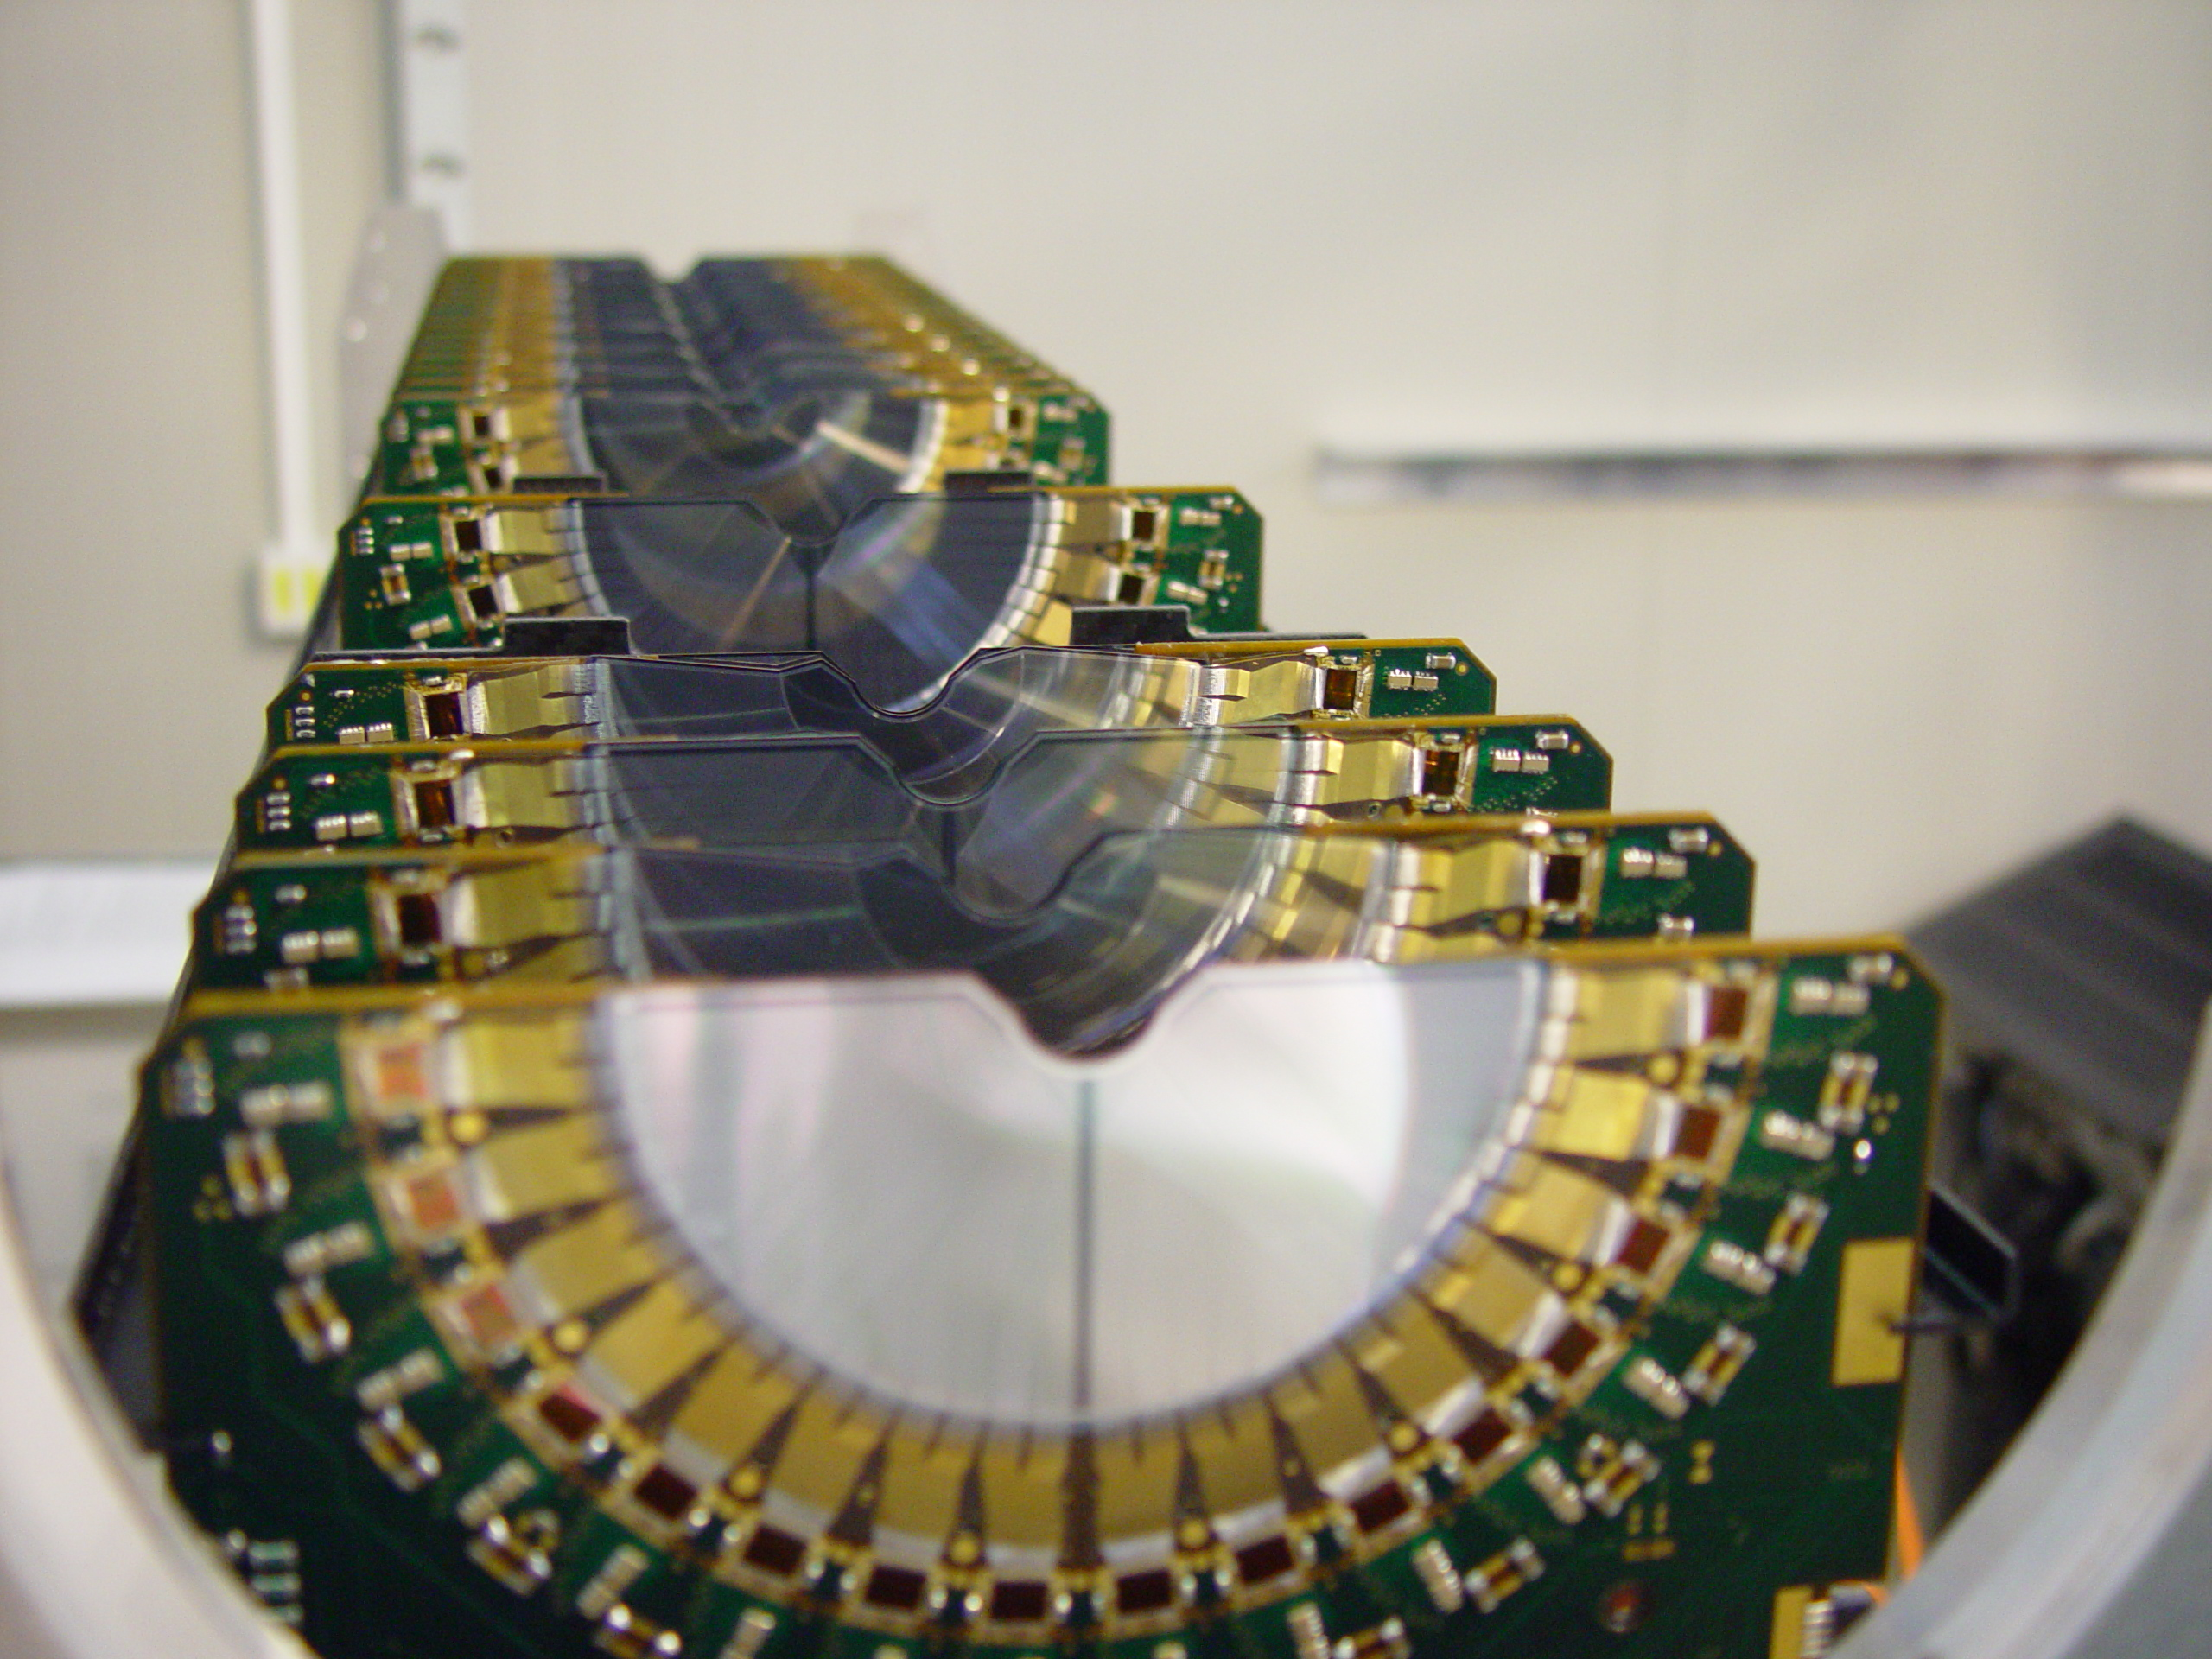
\includegraphics[width=0.5\textwidth]{detector_velo_real}
	\end{center}
	\caption[LHCb's VELO subdetector]{The 26 layers of one half of the VELO. The pixels reside on the silver area, the PCB around contains the reading electronics, and the wedge at the top-center of the silver area is where the beam passes through. \cite{cern_document_server}}
	\label{fig_detector_velo_real}
\end{figure}

The UT (see \ref{fig_detector_ut_ft_drawing}) is a silicon strip detector which consists of long fibers which act much like a pixel as they also signal if a particle passes through them at any point along their length. A fiber of the UT is generally 10 centimeters long, and has a width of only 192 micrometers. This means that while on one axis, the particles position can be told with great accuracy, on the other axis the uncertainty is 10 centimeters. The entire detector measures about 1.7 meters in width and 1.4 meter in height.

Similarly to the UT, the FT is also a silicon strip detector, but the length of its fibers is 2.5 meters. This means the 5 meter tall detector needs only two fibers to cover the full height.

\begin{figure}[H]
	\begin{center}
		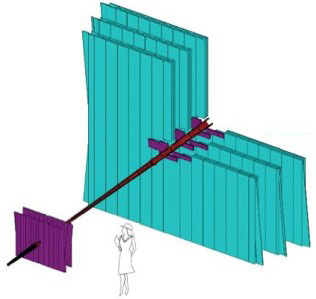
\includegraphics[width=0.5\textwidth]{detector_ut_ft_drawing}
	\end{center}
	\caption[The UT and FT detectors, schematic view]{The UT in purple and the FT in blue, with a person next to them to illustrate the scale. The silicon strips are aligned vertically, leading to a good horizontal resolution but a poor vertical resolution. \cite{tracker_image}}
	\label{fig_detector_ut_ft_drawing}
\end{figure}

In between the UT and the FT, a strong magnet is placed which bends the particles on the horizontal axis.

When a collision occurs, the particles follow a straight path and they are recorded passing through the pixels of the VELO. Initial particle trajectories can be reconstructed by finding hits in the VELO that align to form a straight line. These paths are then linearly extrapolated through the UT, and some of the silicon strips that were lit up by the particles are assigned to the initial trajectories acquired from the VELO. Inside the UT, particles paths are mostly straight, but they already experience a slight bending because of the magnet. From the amount of bending, the particle's momentum can be estimated. As the charged particles pass through the magnet, their trajectory bends, however, the amount of bending is a function of the particle's momentum. With a good momentum estimate, a guess can be given as to where the particle would hit the FT. In the suspected region, the silicon strips of the FT are searched and if the corresponding fibers are found, they are assigned to the particle.

At the end of the process, all the pixels or fibers that were touched by a particle are known, which makes it possible to know the exact path of the particle. The amount of bending from the UT to the FT allows the calculation of the momentum, which, when paired with information from other detectors, such as energy and velocity, makes it possible to identify a particle. (Identification means knowing the name of the particle, such as electron or muon.)


\subsection{Events and triggering}\label{sec_events_trigger}


\subsubsection{Collision events}\label{sec_event_what}

The LHC has 2808 bunches of protons in the accelerator at a time, for both beams. We refer to the collision of two particular bunches as an \textit{event}. Events are completely independent, that is, a bunch-bunch collision only happens after the previous collision's products have been analyzed and flushed from the detector. The time between two subsequent bunches is 25 nanoseconds, which would set the rate of collisions at 40 million per second. In reality, there are some gaps between two adjacent bunches that are a lot longer than 25 nanoseconds. Due to these large gaps, the average rate of collisions is about 30 MHz, but a 40 MHz rate of processing is necessary to go without buffering.


\subsubsection{Real-time reconstruction and triggering}\label{sec_trigger_what}

The vast majority of the 30 million events that occur every second are absolutely uninteresting, with no exotic particles of interest being created. On the other hand, so many events together produce a significant amount of data which is a challenge to store. To reduce the amount of data written to permanent storage, each event is processed in real-time to determine weather it is interesting or not. Uninteresting events are simply dropped, the interesting ones are stored long-term for offline analysis. The act of deciding if an event has to be stored is called \textit{triggering}. The real-time processing of events is a simplified method that relies on the VELO, UT and FT detectors as described previously.


\subsection{The 2019/20 upgrade of LHCb}\label{sec_lhcb_upgrade}

The LHC shuts down for maintenance for two years from the end of 2018. The LHCb detector also undergoes maintenance and upgrade during that time, where the VELO is upgraded and the old TT is entirely replaced by the UT.

The pre-upgrade detector did the real-time event processing in two stages. The first stage employed FPGAs to do a preselection, which cut down the 30 million events per second to roughly 1 million per second. The second stage used a large farm of CPUs to do finer reconstruction and final trigger decision. During the upgrade, however, the FPGAs will be retired, and the CPU farm now has to take the whole load of 30 million events per second. This puts a stress on the software stack that it was not written to handle, and needs a significant overhaul.

\begin{figure}[H]
	\centering
	\begin{subfigure}{.5\textwidth}
		\centering
		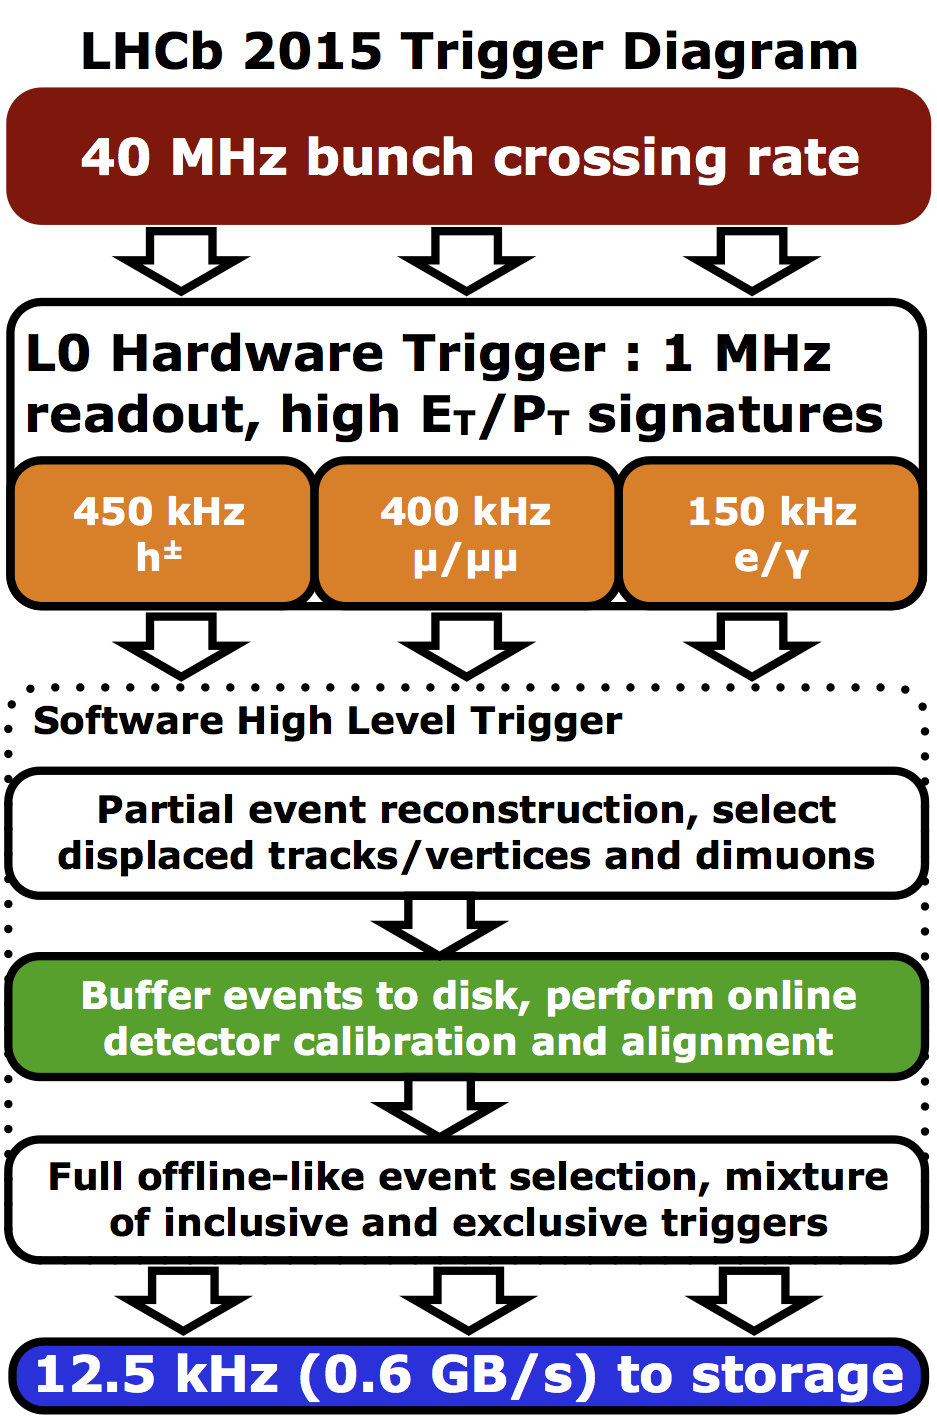
\includegraphics[width=.4\linewidth]{LHCb_Trigger_RunII_May2015}
		\caption{Trigger data flow scheme\\ before the upgrade}
		\label{fig_trigger_compare_sub1}
	\end{subfigure}%
	\begin{subfigure}{.5\textwidth}
		\centering
		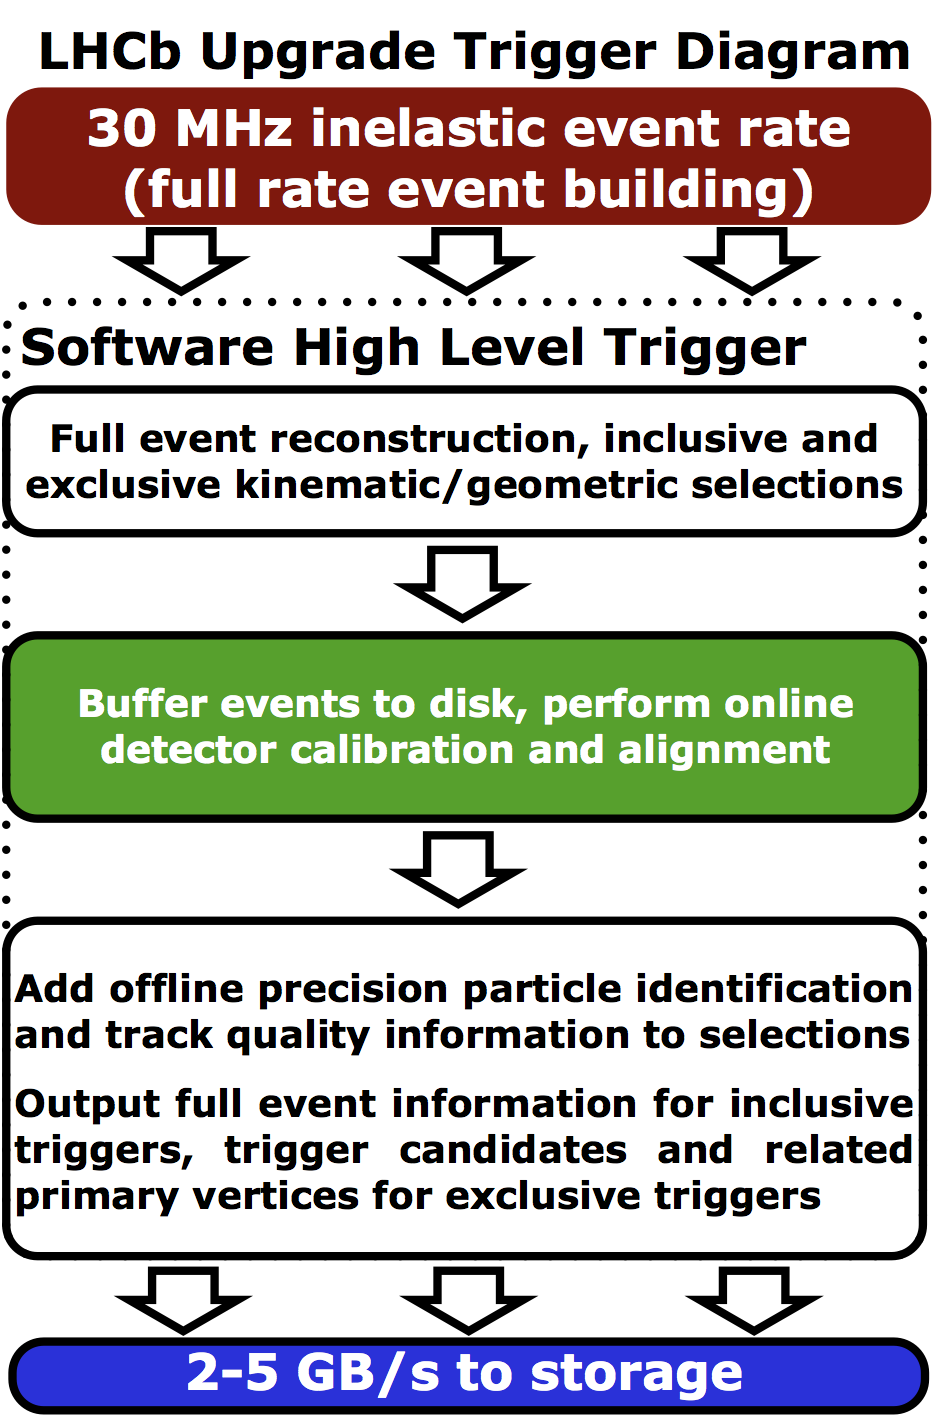
\includegraphics[width=.4\linewidth]{LHCb_Trigger_RunIII_May2015}
		\caption{Trigger data flow\\ scheme post-upgrade}
		\label{fig_trigger_compare_sub2}
	\end{subfigure}
	\caption[Comparison of pre- and post-upgrade triggering]{Comparison of the two triggering solutions. \cite{lhcb_twiki}}
	\label{fig_trigger_compare}
\end{figure}


\subsection{Overview of the real-time processing software}\label{sec_reco_sw_overview}
	
\begin{figure}[H]
	\begin{center}
		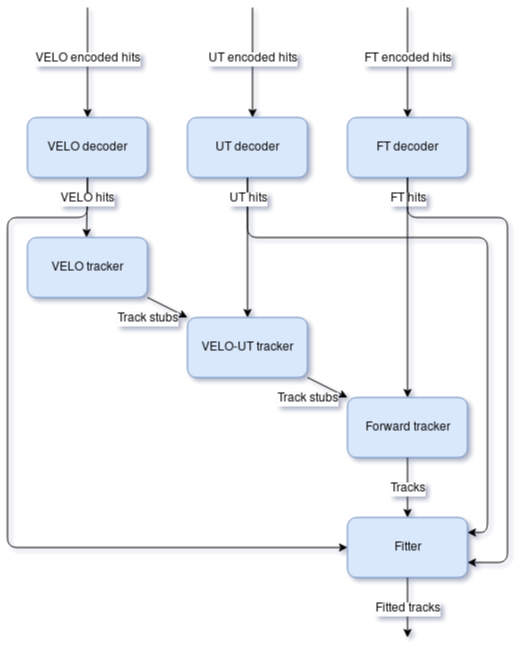
\includegraphics[width=0.6\textwidth]{algorithms_brunel}
	\end{center}
	\caption{Simplified view of algorithms that perform online reconstruction.}
	\label{fig_algorithms_brunel}
\end{figure}

The real-time processing software consists of algorithms which do a specific piece of the reconstruction of the particle paths. In addition to the reconstruction, there are other algorithms which do the selection of interesting events. Since the selection algorithms are generally a lot faster than reconstruction algorithms, they are excluded from this discussion.

The general principle behind reconstruction is that a list of hits (where a pixel or silicon strip was hit) are given, and regular alignment of the hits indicate the path of the particle: hence the name \textit{pattern recognition}. Once all particles have been found by gathering the hits they created, they can be identified and fed into the selection decision making.

The information on which pixels and strips were hit comes straight from the detectors, in a heavily compressed binary format. It has to be first decoded to obtain the position of the individual strips, a process done by the \textbf{VELO decoder}, \textbf{UT decoder} and \textbf{FT decoder}.

Once pixel hit positions are known by their global X,Y,Z coordinates, the \textbf{VELO tracker} finds hits that align to form a straight line. It estimates the starting position and the slope of the line. The line is extended into the UT, where the \textbf{VELO-UT tracker} searches silicon strip hits that are very close to the extended line. From the slight offset of the strip hits from the extended line, the VELO-UT tracker can estimate the amount of bending in the magnetic space, thus the momentum of the particle. The last step of tracking is done by the \textbf{forward tracker}, which uses the momentum estimate to extrapolate the bent path of the particle through the magnet, to the layers of the FT. It then finds silicon strips of the FT which align into a straight line (no magnetic field in the FT either), the line having the right direction and position to be a possible path the particle took after going through the magnet.

Finally, the \textbf{fitter} uses all the hits to align the particles path more closely with the position of the hits. In principle, it works similarly to a curve fitting solution, but uses a Kalman filter\cite{kalman_filter_wiki}\cite{kalman_filter_lhcb} internally. Having the most accurate path for each particle, the decision is made to keep or drop the event. (Note that \textit{fitter} and \textit{filter} are used interchangeably, as the algorithm falls into both categories.)


\subsection{Goals for the upgrade}

\subsubsection{Previous work}

As explained in \ref{sec_lhcb_upgrade}, the abandonment of the hardware trigger stage highly increases the load on the software trigger. To cope with the load in a cost-efficient manner, both a hardware and a software upgrade will take place. Regarding the hardware upgrade, a new computing farm with the latest many-core server processors will be built. This thesis, however, focuses on the software upgrade.

\vspace{1pc}
The majority of the code was written a decade ago, made to perform well in those environments. Since then, hardware changed substantially. The most prominent change is the appearance of many-cores on a single processor die -- up to 40-60 cores as opposed to 2-4 cores back then. It is no longer enough to start a process for each core, because the duplication of shared static memory resources consumes an unacceptable amount of memory. The application was, however, not prepared to efficiently handle multithreading. The gap between CPU speed and memory speeds has grown even more. It is now crucial to use minimalist, cache efficient data structures to avoid being bound by memory. Modern processors also introduced data-parallelism on the instruction level with extensions such as SSE, AVX and AVX-512. Making use of these instruction sets requires special attention to data structures and explicit code on behalf of the programmer. In return, data-parallelism can achieve a performance of up to 16 times higher than that of plain, scalar code*.

\vspace{1pc}
After a determined optimization effort, the team eliminated main bottlenecks from the software, such as excessive locking due to the lack of thread safe design, extremely slow algorithms and pre-computable calculations. Despite that, as of September 2018 (when I began working on this thesis project), a threefold speedup** was still required to achieve the target throughput of 30 million events per second processed. Should the throughput stay below the threshold, unprocessed events will be dropped, reducing the amount of valuable data collected, limiting the physics research potential of the experiment.

\subsubsection{Contributions of this thesis project}

\vspace{1pc}
This thesis project provides solutions to the optimization of three major parts of the code:
\begin{enumerate}
	\item the parameterized Kalman fitter (\ref{sec_kalman_main}),
	\item the data model of the particle path reconstruction algorithms (\ref{sec_datamodel_main}), and
	\item the VELO-UT reconstruction algorithm (\ref{sec_opt_velout}).
\end{enumerate}
The means of optimization are introducing minimalistic, cache efficient data structures, vectorizing code, reducing branching and eliminating heavy/inefficient instructions. Additionally, general code design improvements and code modernization also plays a part in increasing both performance and maintainability. The speedups achieved by this work should help the LHCb collaboration to increase event-processing throughput to the required threshold.

\vspace{1pc}
\small
\noindent\tab* In case of AVX-512, not accounting for downclocking\\
\noindent\tab** Threefold for the best-throughput configuration, the acceptable case; six fold for the best-physics configuration, the ideal case
\normalsize


%----------------------------------------------------------------------------
% === OPTIMIZATION TARGETS ===
%----------------------------------------------------------------------------
\newpage
\section{Choosing optimization targets}

\subsection{The parameterized Kalman fitter}

The software's built-in profiler measures the execution time of individual algorithms.

\begin{figure}[H]
	\begin{center}
		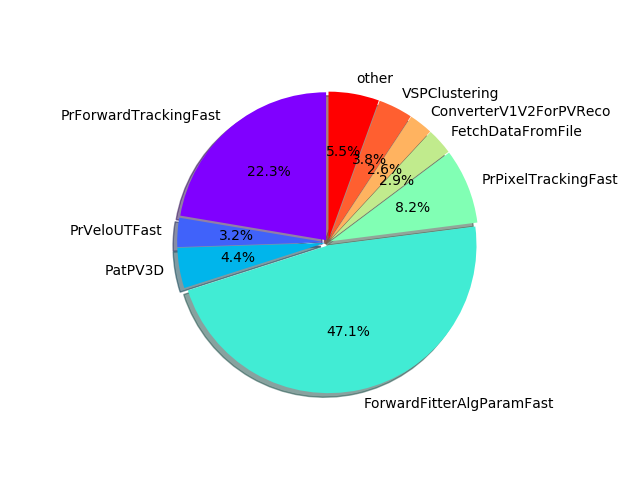
\includegraphics[width=0.6\textwidth]{algo_usage_original_bestphys}
	\end{center}
	\caption{Workload distribution among trigger software algorithms, mid 2018}
	\label{fig_algo_usage_choice}
\end{figure}

Figure \ref{fig_algo_usage_choice} shows the relative CPU time the algorithms take on a pie chart. It can be seen that the largest fraction, 47.1\% is consumed by the parameterized fitter. A deeper analysis into the code of the parameterized fitter using Intel VTune showed that a substantial part of the computation time is spent in trivial calculations that are potentially easy to remove. Providing a very high return on investment, the parameterized fitter was an ideal first target for optimization.


\subsection{The global data model}

Work on the parameterized fitter uncovered serious issues with the classes and data layout of the particle path reconstruction and refinement algorithms. Additionally, work on the fitter was incomplete as it polluted the already-convoluted data model even more. Fixing the data model to be cache friendly, to support the vectorization of the algorithms and to avoid deep copies throughout the reconstruction pipeline was a natural choice.


\subsection{The VELO-UT algorithm}

Having the vectorization friendly data model in place, the rest of the team was already busy vectorizing the particle path reconstruction. The VELO-UT algorithm was still awaiting the overhaul, and as it was the remaining non-vectorized top consumer, I took on the task. The work was expected to increase code maintainability by replacing the aging and cluttered code, as well as to provide substantial speed improvements.


%----------------------------------------------------------------------------
% === PARAMETRIZED KALMAN ===
%----------------------------------------------------------------------------
\newpage
\section{Parameterized Kalman Fitter}\label{sec_kalman_main}

As described in \ref{sec_reco_sw_overview}, the track is reconstructed incrementally, start with VELO hits, extended by UT hits and finally adding the FT hits. This process, however, is not so accurate. This manifests itself in the creation of \textit{ghost tracks} and missed tracks, and generally, tracks are only roughly aligned with the hits they were made from. Ghost tracks are tracks that did not exist in the real collision, they are merely artifacts of the reconstruction algorithms. As such, ghost tracks are highly undesirable, but the Kalman fitter helps to weed them out. 
The Kalman fitter basically refines the rough tracks that are spit out by preceding algorithms. The state of a particle can be described by its position, direction, and the quotient of its charge and momentum. The Kalman fitter first estimates the particle's state at its birth position based on the VELO hits alone. After that, it extrapolates the state of the particle to the next hit, or in other words, simulates the particle's travel until the next hit using the laws of physics. The new, \textit{predicted} state will have some deviation from the \textit{observed} state (that is, the hit), however, the Kalman fitter can make a mathematically optimal estimate for the true state based on the prediction and observation. The very new optimal state estimate will then be extrapolated to the next hit again, and this repeats for all the hits of the track.
As a result, the estimated state or path of the particle aligns more closely with the observed hits. In the case of ghost tracks, we can expect to have large deviations between the optimal estimated states and the observed hits, which could have slipped through initial reconstruction algorithms but show up for the fitter. Such tracks are removed from the list of tracks, and that's why fitting is important.


\subsection{Performance profiling for hotspots in the Kalman fitter}

\begin{figure}[H]
	\begin{center}
		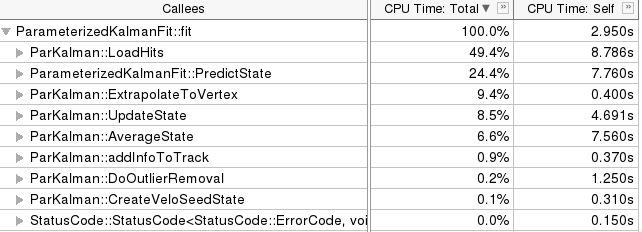
\includegraphics[width=0.9\textwidth]{kalmanfit_overall_breakdown}
	\end{center}
	\caption[CPU hotspots in the Kalman fitter]{Hotspots, or which parts of the Kalman fitter takes most of the time. Measured by Intel VTune Amplifier XE.}
	\label{fig_kalman_vtune_initial}
\end{figure}

Figure \ref{fig_kalman_vtune_initial} shows what fraction of the CPU time is spent in individual functions of the Kalman fitter's code. We can nicely see how the theoretical steps of the Kalman fitting map to the functions:
\begin{itemize}
	\item LoadHits: acquires position and measurement error of hits
	\item PredictState: extrapolates the state to the next hit
	\item UpdateState: makes an optimal estimate for the true state using the predicted state and the measured hit
	\item AverageState, ExtrapolateToVertex, etc.: various operations
\end{itemize}
There is a major and obvious problem however: just acquiring the data on which the computation is done should not take over 50\% of the Kalman fitting, but more like 1\%.	


\subsection{Loading hits in detail}

Careful examination reveals the way hits are loaded through the so-called \textit{Measurement providers}.
	
\begin{figure}[H]
	\begin{center}
		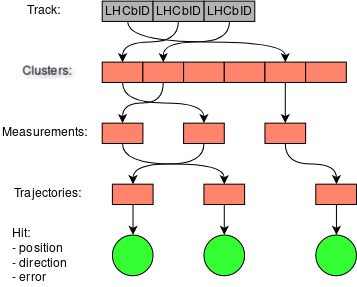
\includegraphics[width=0.6\textwidth]{kalmanfit_loadhits_schematic}
	\end{center}
	\caption[Loading of track data from LHCbIDs]{Illustration of how hit information is acquired from the array of LHCbIDs stored inside the Tracks. Contiguous array of clusters correspond to contiguous DRAM memory regions, while distinct objects, i.e. measurements have no spatial locality.}
	\label{fig_kalmanfit_loadhits_schematic}
\end{figure}

When a particle hits a detector, the identifier of the element of the detector that was hit is recorded. (Detector elements are analogous to the pixels of a digital CCD camera.) These elements are basically unambiguously identified by the so-called \textit{LHCbIDs} (represented by an integer), so it is enough to store the IDs inside the Track object and all information (such as location of the hit, measurement error) can be recovered. 

Over the years however, this system grow unnecessarily complex resulting in a dramatic slowdown. Clusters, containing some basic information about the hit, such as its location, are stored inside measurement providers as a large array. In order to find the cluster that corresponds to the ID, this whole array is searched linearly. Once the cluster is found, a \textit{Measurement} object is allocated on the heap and initialized from it. Finally, another object, called a \textit{trajectory}, is queried from the measurement, from which the data actually required can be extracted. The storage of clusters and creation of measurements is handled by \textit{MeasurementProviders}. Additionally, we can distinguish separate measurement objects for the VELO, UT and FT hits.

As seen, this is a convoluted process, involving an asymptotically unacceptable linear search and a lot of dynamic memory allocation. Dynamic allocation is not only slow, it highly suffers from thread contention at the operating system level in our multi-threaded software. Additionally, the individually allocated objects are scattered around in memory, resulting in poor CPU cache performance.

\begin{figure}[H]
	\begin{center}
		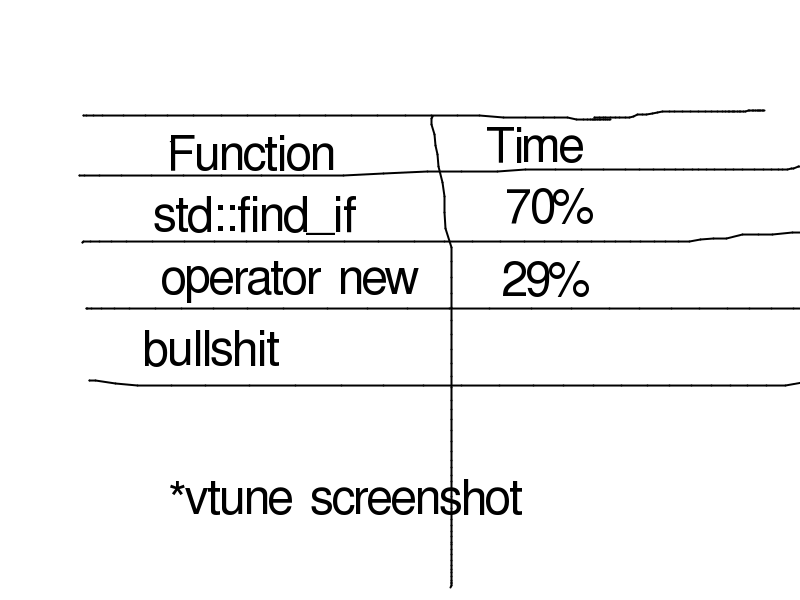
\includegraphics[width=0.9\textwidth]{kalmanfit_loadhits_breakdown}
	\end{center}
	\caption{Breakdown of CPU usage of the LoadHits function}
	\label{fig_kalmanfit_loadhits_breakdown}
\end{figure}

Figure \ref{fig_kalmanfit_loadhits_breakdown} shows an excerpt from the CPU profiler and helps to understand where LoadHits spends its time. The most obvious thing is the \code{std::find\_if}s that take nearly 60\% of LoadHits. This is the function that does the linear search among clusters. The rest of the overhead comes from various boilerplate code, clear trends cannot be understood, but the volume of the overhead is seen to be significant.


\subsection{Simplifying the data loading}

To avoid this long chain to acquire the required data, the hits should be directly stored inside the Track rather than only by their IDs. Ideally, this would not incur any performance penalty, since the algorithms preceding the Kalman fitter all use the position and error information associated with a hit, so the detector element identifier is fully decoded anyway.

As described, the Track object has the following content (largely simplified):
\begin{lstlisting}[language=C++]
	struct Track {
		std::vector<LHCbID> ids;
	};
\end{lstlisting}

In the new model, the following structure is used:
\begin{lstlisting}[language=C++]
	struct TrackHit {
		Vector3D beginPosition;
		Vector3D endPosition;
		float errorX;
		float errorY;
	};
	
	struct Track {
		std::vector<LHCbID> ids;
		std::vector<TrackHit> veloHits;
		std::vector<TrackHit> utHits;
		std::vector<TrackHit> ftHits;
	};
\end{lstlisting}

Notice how the IDs are kept: the unfortunate reason for this is that other algorithms rely on these, and they cannot be removed in this first iteration. This structure, however, completely eliminates clusters, measurement and trajectories from the chain, and the Kalman fitter reads the contiguously stored information straight out of the track. This does not stress the memory allocator and is friendly for the caches.


\subsection{Performance profiling of the simplified model}

\begin{figure}[H]
	\begin{center}
		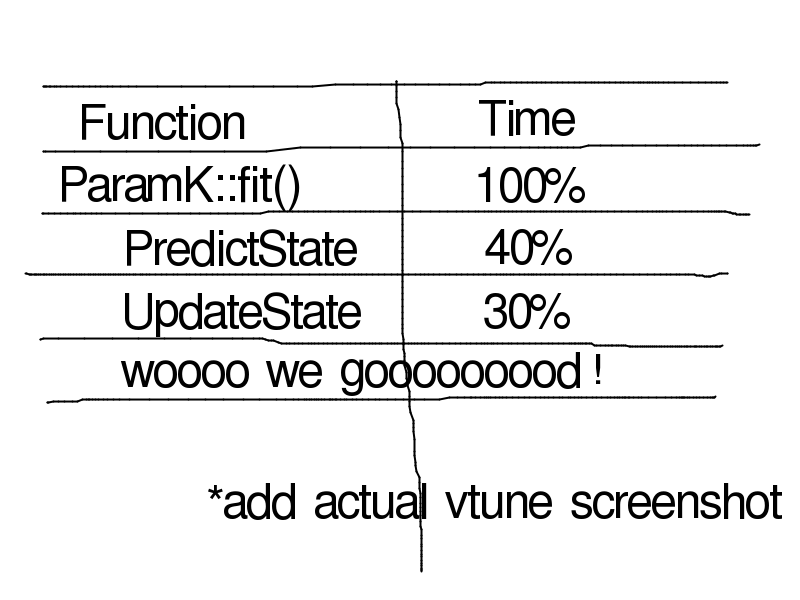
\includegraphics[width=0.9\textwidth]{kalmanfit_simplified_overall_breakdown}
	\end{center}
	\caption[CPU hotspots of the Kalman fitter after optimization]{Breakdown of the Kalman fitter after the simplified data loading}
	\label{fig_kalmanfit_simplified_overall_breakdown}
\end{figure}

Figure \ref{fig_kalmanfit_simplified_overall_breakdown} shows that with the new data model, the previous CPU hog, LoadHits, has completely disappeared, now accounting only for 1.2\% of the fitting.

As the parametrized Kalman fitter takes about 47\% of the entire reconstruction sequence, and about 50\% of the fitter's computing load was removed by the above described code changes, we would expect an overall speedup of 31\%. When measured, throughput increases from 4450 events processed per second to about 4850 events/second, or about 9.2\%. As this is way less than the predicted 31\%, the question arises as to where the performance is gone. First of all, three new data members were added to the Track to store the new TrackHits, and nothing has been removed. As Tracks are copied in the code, the three std::vectors also have to be copied, which involves dynamic memory allocation (a well-known performance drag) and memory copying. Second, part of the code that produces the TrackHits from other objects was not removed, but merely moved out of the fitter to other algorithms. The data conversion to TrackHits, along with adding the TrackHits to the vectors and allocating the memory of the vectors adds additional overhead. In order to achieve the projected performance improvements, these issues have to be fixed and optimized.


\subsection{High level optimizations}

Besides the TrackHits (or IDs), the Track contained three additional dynamically allocated \code{std::vectors}, which were filled with valid data but were not necessary from a computing point of view. Removing these data members confirmed the hypothesis by which the additional data members in the track slowed down the algorithm sequence: I observed an increase of 17\% in throughput (on top of the 9.2\%) when removing these members. While this can be regarded as an optimization independent to the fitter itself, it gains back the speed lost with the additional members required by the fitter.


\subsection{Micro-optimizations}

To trade physics quality for performance, event culling decisions can be made earlier in the reconstruction sequence, before fitting. This results in fitting taking a lot smaller part of the entire sequence while other algorithms become more prevalent. My work, although sped the fitting up, slightly slowed other algorithms down. Consequently, the \textit{best physics} case experienced a large increase in throughput, but the \textit{best throughput} case got slightly slowed down. In an attempt to restore the performance of the other algorithms, I had to further analyze performance.

\begin{figure}[H]
	\begin{center}
		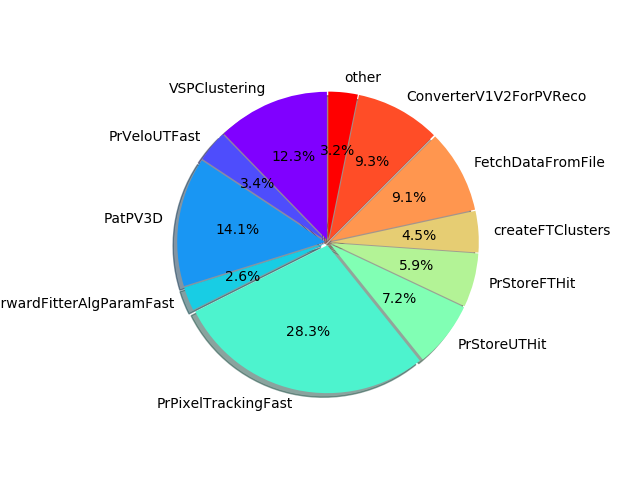
\includegraphics[width=0.6\textwidth]{algo_usage_original_bestthru}
	\end{center}
	\caption{Distribution of CPU time among algorithms in the \textit{best throughput} case with early event culling}
	\label{fig_algo_usage_original_bestthru}
\end{figure}

Figure \ref{fig_algo_usage_original_bestthru} shows the best throughput case where the pixel tracking algorithm takes the most amount of time. This algorithm is responsible for finding particle track stubs from only VELO hits, and was negatively affected by my fitter optimizations.

\begin{figure}[H]
	\begin{center}
		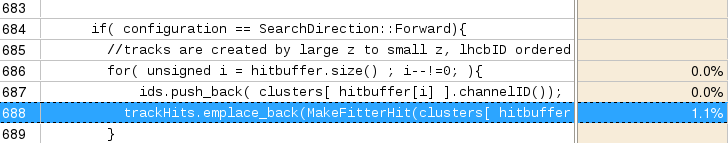
\includegraphics[width=0.9\textwidth]{kalmanfit_disasm_opt_src_naive}
	\end{center}
	\begin{center}
		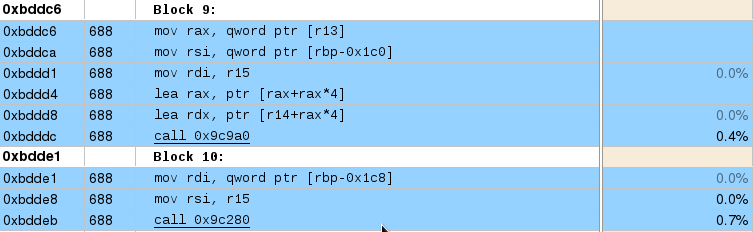
\includegraphics[width=0.9\textwidth]{kalmanfit_disasm_opt_asm_naive}
	\end{center}
	\caption[Undesired code growth from the fitter optimization]{Code snippet from the profiler which shows the code I added to the pixel tracking algorithms in blue highlight. The upper image shows the C++ source code, the lower image shows the corresponding x86-64 disassembly.}
	\label{fig_kalman_disasm_src_naive}
\end{figure}

Looking at the disassembly, we can see two \textit{CALL} instructions, which correspond to the two function calls \textit{MakeFitterHit} and \textit{emplace\_back}. This means that the functions haven't been inlined. Inlining is a complex topic, because it can make code faster by removing function prologues, but excessive inlining can also make code slower by polluting the instruction caches with too many repeated code snippets. In this case, the latter is unlikely, since these function are only present at this location, so inlining would be preferable.

\begin{figure}[H]
	\begin{center}
		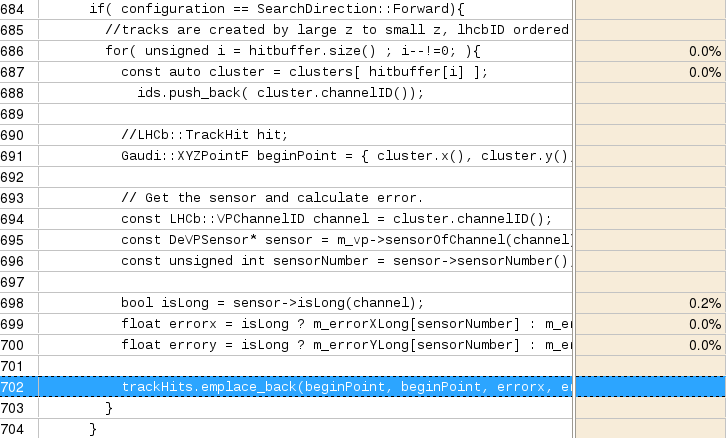
\includegraphics[width=0.9\textwidth]{kalmanfit_disasm_opt_src_inlined}
	\end{center}
	\begin{center}
		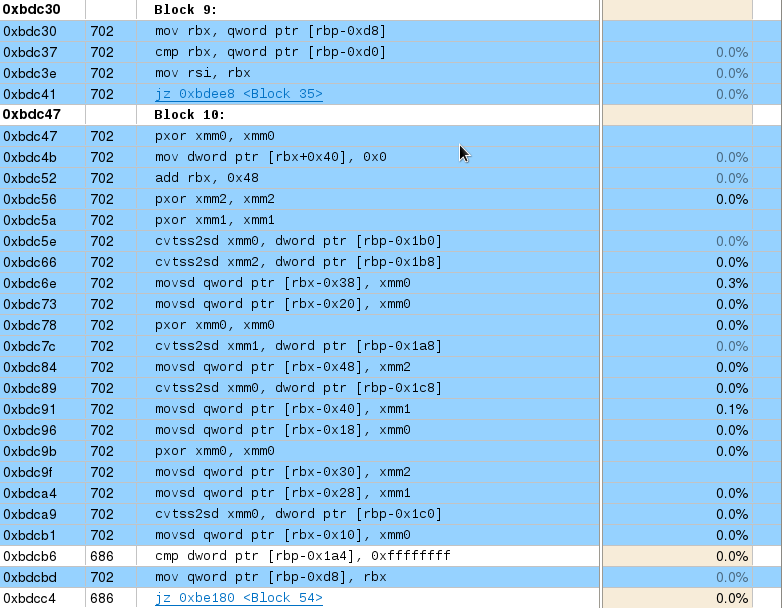
\includegraphics[width=0.9\textwidth]{kalmanfit_disasm_opt_asm_inlined}
	\end{center}
	\caption[Code growth performance mitigated]{Source code and disassembly after manually inlining \textit{MakeFitterHit} inside the \textit{for} loop.}
	\label{fig_kalman_disasm_src_inlined}
\end{figure}

As can be seen on figure \ref{fig_kalman_disasm_src_inlined}, both \textit{CALL} instruction have disappeared. The first one for \textit{MakeFitterHit} due to the manual inlining, and the second for \text{emplace\_back} because of the compiler automatically inlining it. Note that the automatic inlining was enabled by passing the constructor arguments of \textit{TrackHit} to \textit{emplace\_back} instead of the ready object, exactly as \textit{emplace\_back} was meant to be used. Now, theoretically, the compiler could optimize out both cases as their semantics are equivalent, but it is apparently not capable of doing so.

Besides the absence of function calls, there is another thing noticeable on the assembly instruction. There is a large number of instructions moving quad words (\textit{MOVSD}), that is 64 bit double precision numbers. Furthermore, the \textit{CVTSS2SD} instructions are converting 32 bit single precision numbers to 64 bit doubles. Looking at the source code, we can indeed notice that input data from which the \textit{TrackHit} is made is stored as single precision floats, but the \textit{TrackHits} themselves are double precision because the fitter is using double precision calculations. Changing \textit{TrackHit} to store single floats as well, thus delaying the conversion, will hurt performance at another place where it has less of an impact.

\begin{figure}[H]
	\begin{center}
		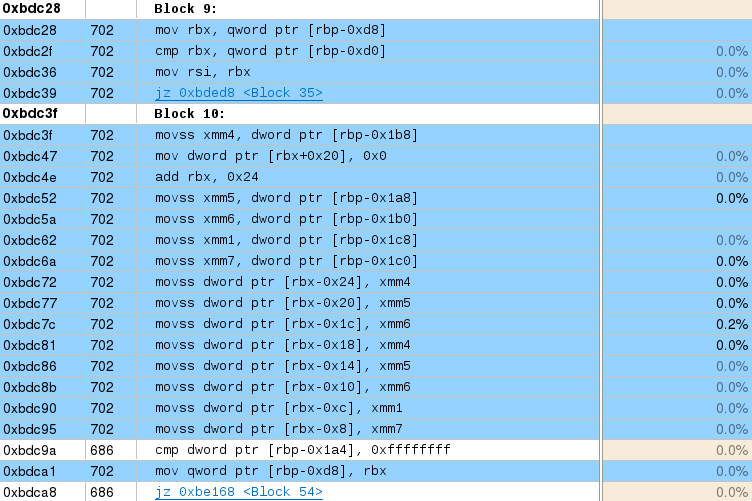
\includegraphics[width=0.9\textwidth]{kalmanfit_disasm_opt_asm_nocvt}
	\end{center}
	\caption{Disassembly after changing \textit{TrackHits} to store single floats.}
	\label{fig_kalman_disasm_src_nocvt}
\end{figure}

The disassembly on figure \ref{fig_kalman_disasm_src_nocvt} clearly shows that the single precision to double precision conversions are gone just like the \textit{PXOR} instructions, and now it only moves double word memory units. With this little change, I managed to throw out lots of unnecessary instruction and the amount of memory moved around is also smaller.

Due to the complex interactions inside modern, pipelined CPUs and between the CPU, the DRAM and caches, it is hard to explain how and why the changes affected the performance. Nevertheless, inlining and trimming the assembly code has increased performance of the \textit{best throughput} scenario with early event culling from 13300 events per second to around 13700. Notably, the basic case without my code changes has produced about 14500 events per second. \small (As measured with my development branch on our performance test machines during development.) \normalsize


\subsection{Results, conclusion}

I managed to significantly increase the throughput of the \textit{best physics} case from 4450 events per second to 5870 events per second, or a 32\% increase. Unfortunately, the \textit{best throughput} case slowed down from 14500 events/sec to about 13700, or 5\% decrease in throughput. The speedup can be explained by removing unnecessary work by simplifying the code. The slowdown of the \textit{best throughput case} can be attributed to overall making the \code{Track} object slightly heavier and its creation more expensive, and the reduced weight of the code that got faster can't make up for it anymore. This is still acceptable, however, as the modifications to the \code{Track} are only temporary and should disappear with future clean-up and refactoring of the data model.

\begin{figure}[H]
	\begin{center}
		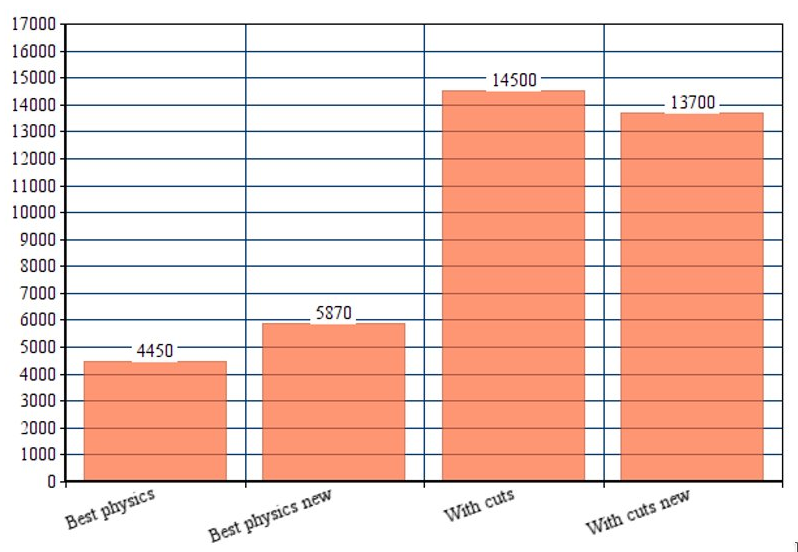
\includegraphics[width=0.7\textwidth]{kalmanfit_throughput_results_lowquality}
	\end{center}
	\caption[Throughput improvement by the Kalman fitter optimization]{Throughput of the particle path reconstruction before and after my modifications, for the \textit{best physics} and \textit{best throughput} cases.}
	\label{fig_kalmanfit_results_throughput}
\end{figure}

Another interesting figure to look at is how the weight of the parameterized Kalman fitter in the entire algorithm sequence has changed. Previously, it took 47\% of the whole sequence, and now it only takes 22\%. If in addition the fact that the whole sequence is significantly faster is factored in, the fitter is well above two times faster. \small (These type of measurements are to be taken with a grain of salt because of complex system interactions and the consequent inaccuracy of profiling, but are interesting and provide a good general view.) \normalsize

\begin{figure}[H]
	\centering
	\begin{subfigure}{.5\textwidth}
		\centering
		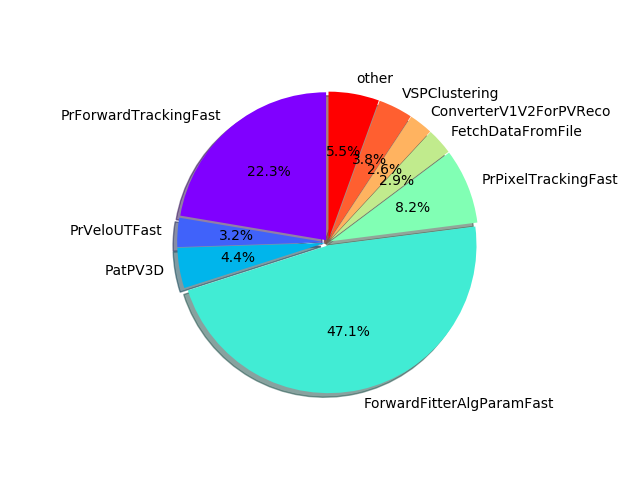
\includegraphics[width=\linewidth]{algo_usage_original_bestphys}
		\caption{Before optimizations}
	\end{subfigure}%
	\begin{subfigure}{.5\textwidth}
		\centering
		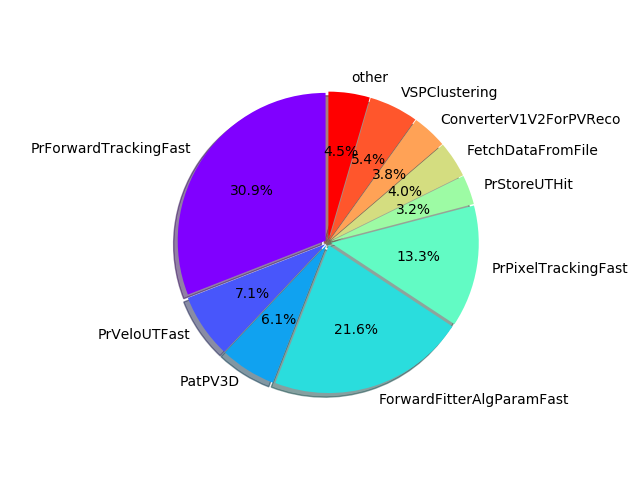
\includegraphics[width=\linewidth]{algo_usage_optkalman_bestphys}
		\caption{After optimizations}
	\end{subfigure}
	\caption[CPU time share of algorithms after Kalman fitter optimizations]{The distribution of processor time requirements of each algorithms. The parameterized Kalman fitter is identified by the label \textit{ForwardFitterAlgParamFast}.}
	\label{fig_kalmanfit_results_algousage}
\end{figure}

In light of the code changes and their effect on the overall performance, we can safely say that code should strive to do the data transformations in the simplest possible way. Adding extra layers on top, if not done carefully using zero-cost abstractions, will dramatically slow the code down. In performance critical applications, a good data oriented design can give far better benefits than assembly-level micro-optimizations. Additionally, a good data structures opens up the doors to more effective micro-optimizations, such as vectorization.


%----------------------------------------------------------------------------
% === DATA MODEL ===
%----------------------------------------------------------------------------
\newpage
\section{Streamlining the computation's data model}\label{sec_datamodel_main}

While profiling the Kalman filter, I had to change the data model by adding additional data to the \code{Track} which had adverse effects on performance (see \ref{sec_kalman_main}). As the changes were temporary, the performance issue wasn't a concern, but the general performance of the data model was. Over the years the code accumulated quite some unnecessary data and code which resulted in issues with performance and maintainability. This chapter explains how data structures can be streamlined to better accomodate modern computer architectures.

\subsection{The existing data model}

The algorithms that constitute the processing chain are illustrated on figure \ref{fig_algorithms_brunel}. There are two main categories of data passed from one algorithm to the other: hits and tracks. All data related to a track is represented by the \code{Track} class, and in general, \code{std::vector}s of \code{Track}s are passed from one algorithm to the next. The \code{Track} was designed to be a generic object that is able to represent all the different types of tracks, for example a \textit{VELO track} or a \textit{forward track}.

\begin{lstlisting}[language=C++,caption=Simplified code of the \code{Track} class.,label=lst_datamodel_trackv2_simple
]
	class Track {
		/* ... */
	private:
		std::vector<LHCbID> lhcbIDs;
		std::vector<State> states;
		std::vector<Track*> ancestors;
		std::map<int, double> extraInfo;
		std::vector<Measurement*> measurements;
		std::vector<Node*> nodes;
	};	
\end{lstlisting}

In case of the trigger software, all tracks begin with the VELO. The VELO tracker finds hits that are aligned in a straight line and creates a \textit{VELO track} that is then forwarded to the VELO-UT tracker. The so called \textit{VELO tracks} contain the IDs of the pixels that were hit in the VELO detector, as well as the estimated state of the particle at its birth and when it left the VELO. Similarly, the VELO-UT tracker appends the IDs of the UT hits that it found as well as an additional state of the particle inside the UT detector.


\subsection{Connection of the data model and the algorithms}

Multiple algorithms have their own internal data structures for their computations, including special track objects, hit objects and particle states. In all cases, however, the generic input \code{Track} has to be converted to these internal data structures, which incurs an unnecessary overhead. The faster the algorithm itself gets, the larger in proportion the conversion overhead. The main tool to speed up algorithms is vectorization, which requires highly specialized data structures to be efficient, therefore requiring careful tuning of the general data layout to avoid conversion.

\subsection{Issues with the existing model}\label{sec_datamodel_issues}

\subsubsection{Overgeneralization and code bloat}

The \code{Track} object was meant to store every kind of track for any purpose. It is used by all the tracking algorithms, including the VELO, UT and FT tracking. Additionally, it contains derived values of the tracking, such as the estimated particle states, but also information related to final fitting. Most algorithms, however, access only a small fraction of this data, and make expensive checks to verify if the particular data they need is inside the \code{Track}. The \code{Track} is a prime example of the \textit{god class} anti-pattern\cite{god_class_wiki}, which in this case not only compromises code quality but also negatively affects performance due to its heavy weight.

\subsubsection{Memory allocations}

The code snippet \ref{lst_datamodel_trackv2_simple} shows only the heavy members of the \code{Track}. The \code{extraInfo}, \code{measurements} and \code{nodes} members are completely unused for the trigger, so they don't amount to any dynamic memory allocation, but they still amount to about 100 bytes of unused data (depending on implementation). The remaining members are actually used, each of them holding dynamically allocated memory. While the IDs and ancestors are only vectors of simple integer data, a \code{State} contains about 80 bytes.

\subsubsection{Expensive copies}

Due to the framework's implementation, each algorithm writes its output (a \code{vector} of \code{Track}s) into an immutable storage. Since the \code{Track} was intended to be mutated by the algorithms, each algorithm has to make a copy of the immutable storage. Because of the several dynamic allocations for each \code{Track} and the sheer size of the members and dynamically allocated storage, the copying takes a significant amount of time.

\subsubsection{Inefficient memory access patterns}

Dynamically allocated memory reduces spatial locality of the data, which pollutes the CPU cache when an entire cache block is loaded for a much smaller piece of data. Additionally, lack of locality increases the chance of cache misses and disables prefetching techniques, negatively affecting performance. In this particular case, locality is an issue on the level of an individual \code{Track} which stores its data in dynamically allocated blocks and also on the level of the vector of \code{Track}s, which could have a structure of array (SOA) layout to store the \code{State}s of all tracks in the same vector.

\subsubsection{Cannot be vectorized}

To achieve maximum performance, it is necessary to make use of the SIMD capabilities of modern CPUs. Vectorization inherently works on SOA data structures, so it makes sense to have the data laid out in that scheme by default. With the current model, one would have to access the first state's $x$ coordinate for 8 consecutive tracks and load them into a vector register to allow for vectorized calculations. This takes 8 memory accesses to non-contiguous locations to fetch the pointers to the vector of states, then another 8 memory accesses to fetch the actual x coordinates. This conversion takes significantly longer than the entire calculation, hiding all the profits of vectorization.


\subsection{Proposed model}

\subsubsection{Hits}

Before getting to the \code{Track} object, the structures representing the hits had to be refactored. Generally, there were 3 different hit \code{class}es, one for the VELO hits, one for the UT hits and one for the FT hits.

\begin{lstlisting}[
	language=C++,
	label=lst_datamodel_uthit_original,
	caption=The original class definition for UT hits.]
class Hit final {
public:
	Hit(LHCb::UTChannelID chanID, unsigned int size, bool highThreshold, double dxDy, double xat0, double zat0, double yBegin, double yEnd, double cos, double error, unsigned int strip, double fracStrip) { ... }

	float cos() const { return m_cos; }
	float cosT() const { return (fabs(m_xAtYEq0) < 1.0E-9) ? 1. / std::sqrt(1 + m_dxDy * m_dxDy) : cos(); }
	float dxDy() const { return m_dxDy; }
	bool highThreshold() const { return m_highThreshold; }
	bool isYCompatible(const float y, const float tol) const { return yMin() - tol <= y && y <= yMax() + tol; }
	bool isNotYCompatible(const float y, const float tol) const { return yMin() - tol > y || y > yMax() + tol; }
	LHCb::LHCbID lhcbID() const { return LHCb::LHCbID(m_chanID); }
	LHCb::UTChannelID chanID() const { return m_chanID; }
	int planeCode() const { return 2 * (m_chanID.station() - 1) + (m_chanID.layer() - 1) % 2; }
	float sinT() const { return tanT() * cosT(); }
	int size() const { return m_size; }
	float tanT() const { return -m_dxDy; }
	float weight() const { return m_weight * m_weight; }
	float error() const { return 1.0f / m_weight; }
	float xAt(const float globalY) const { return m_xAtYEq0 + globalY * m_dxDy; }
	float xAtYEq0() const { return m_xAtYEq0; }
	float xAtYMid() const { return m_x; }
	float xMax() const { return std::max(xAt(yBegin()), xAt(yEnd())); }
	float xMin() const { return std::min(xAt(yBegin()), xAt(yEnd())); }
	float xT() const { return cos(); }
	float yBegin() const { return m_yBegin; }
	float yEnd() const { return m_yEnd; }
	float yMax() const { return std::max(yBegin(), yEnd()); }
	float yMid() const { return 0.5 * (yBegin() + yEnd()); }
	float yMin() const { return std::min(yBegin(), yEnd()); }
	float zAtYEq0() const { return m_zAtYEq0; }
	unsigned int strip() const { return m_strip; }
	double fracStrip() const { return m_fracStrip; }
	int pseudoSize() const;

private:
	float m_cos;
	float m_dxDy; ///< The dx/dy value
	float m_weight; ///< The hit weight (1/error)
	float m_xAtYEq0; ///< The value of x at the point y=0
	float m_yBegin; ///< The y value at the start point of the line
	float m_yEnd; ///< The y value at the end point of the line
	float m_zAtYEq0; ///< The value of z at the point y=0
	float m_x;
	LHCb::UTChannelID m_chanID;
	unsigned int m_size;
	bool m_highThreshold;
	unsigned int m_strip;
	double m_fracStrip;
};
\end{lstlisting}

As it can be seen on code example \ref{lst_datamodel_uthit_original}, these were full-fledged classes which accumulated quite some cruft over the years, having unused data members and a long list of trivial and less trivial methods. The requirements for the hit classes are the same as for the track: plain old data objects that can be represented in an SOA format for efficient vectorization. Additionally, it is very important to keep the size of these objects to the minimum because there are a large number of hits and they are heavily used in computations.

\vspace{1pc}

Without further explanation of the original data members, this class can be reduced to the following:

\begin{lstlisting}[
	language=C++,
	label=lst_datamodel_uthit_simple_aos,
	caption=Plain old data array of structure format for UT hits.]
struct {
	float x0;
	float y0;
	float z0;
	float y1;
	float dxdy;
	float error;
	uint32_t id;
};
\end{lstlisting}

Despite the reduction in code size, the simplified structure is enough for the VELO-UT tracker to perform its task. The structure is a minimal representation of a UT silicon strip in 3D space: contains the 
$\begin{bmatrix}
	x_0 & 0 & z_0
\end{bmatrix}$
starting point, the $[y0, y1]$ interval that represents the two ends of the fiber and the $dx/dy$ slope of the fiber. Note that the fiber is almost vertical (aligned with the Y axis), in same cases tilted slightly by a Z-axis rotation, so these parameters are valid and precise in all cases. The error represents the uncertainty of the particle due to the fiber's width and the ID is a unique identifier for each fiber.

\vspace{1pc}

A similar scheme can be applied to both the VELO and the FT hits.


\subsubsection{Tracks}

First, we have to realize that the original \code{Track} class breaks the single responsibility principle by representing multiple objects of multiple purposes under the same class. Second, the only thing that's necessary from the \code{Track} object illustrated in code snippet \ref{lst_datamodel_trackv2_simple} is the \code{LHCbID}s (or hits), the \code{State}s and the information as to which UT track came from which VELO track (\code{ancestors}).

In light of this, it makes sense to separate the states and the sets of hits into two separate \code{vector}s of the same size, and the output of the VELO tracking algorithm becomes
\begin{lstlisting}[language=C++]
std::tuple<
	std::vector<VeloTrack>,
	std::vector<State>
>;
\end{lstlisting}
where a \code{VeloTrack} is defined as 
\begin{lstlisting}[language=C++]
struct VeloTrack {
	std::vector<VeloHit> veloHits;
};
\end{lstlisting}

Note that there is no need for separately specifying the \code{LHCbID}s as the \code{VeloHit}s contain them along with all the other information about the hit that is necessary for later analysis of the track.

\vspace{1pc}

Similarly, we can define further types of tracks:
\begin{lstlisting}[
	language=C++,
	label=lst_datamodel_ut_ft_tracks,
	caption=The UT (\textit{upstream}) and FT \textit{long} tracks also contain a reference to the track they were extended from.]
struct UtTrack {
	std::vector<UtHit> utHits;
	const VeloTrack* veloSegment;
};
struct FtTrack {
	std::vector<FtHit> ftHits;
	const UtTrack* utSegment;
};
\end{lstlisting}

The algorithms and their input and output are best illustrated with a graph. The decoders return a plain vector of hits. The tracking algorithms operate on the track stubs and the hits, and write out the extended tracks and the estimated states of the particle. Note that since the \code{Track} and are split, the VELO-UT tracker is able to consume only the particular states that it needs.

\begin{figure}[H]
	\begin{center}
		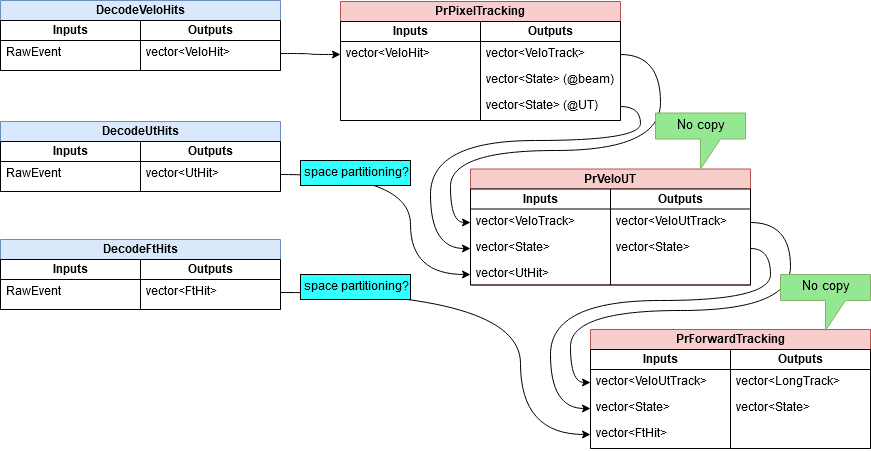
\includegraphics[width=1\textwidth]{datamodel_track_flow}
	\end{center}
	\caption{Algorithms and data flow with the simplified data model.}
	\label{fig_datamodel_track_flow}
\end{figure}


\subsection{Results}

\subsubsection{Problem mitigation}

As explained in \ref{sec_datamodel_issues}, there were several issues with the original data mode.

\vspace{1pc}
As it can be seen on the code snippets, the amount of code has been greatly reduced. Most notably, trivial getter and setter methods have been replaced by public members, and non-trivial getters have been extracted to free functions to where they are needed. Code that is not used in the context of the trigger or tracking has been removed permanently.

\vspace{1pc}
The number of memory allocations was somewhat reduced. The states are now stored in a contiguous array instead of one dynamic block for every track, and the ancestors have also been restructured to be implicit to the track types instead of a dynamically allocated vector per track. Hits, however, are still reside in per-track heap storage.

\vspace{1pc}
Copies of dynamically allocated objects have been eliminated, since when an algorithm extends an existing track it stores a pointer to it along with the new track instead of making a copy of the track and modifying it with the extended parts.

\vspace{1pc}
Memory access patterns are slightly better, as the states reside in a large contiguous chunk of memory. In practice, this unfortunately does not help as the algorithms don't process all states in a tight loop, but rather on a more on-by-one basis. Additionally, algorithms still use only about one third of the data in states.

\vspace{1pc}
Thanks to the plain old data (POD) structures, vectorization is easier, however it still requires deinterleaving the arrays of structures (AOS). Fortunately, POD AOS layouts are fairly easy to turn into SOA layouts.


\subsubsection{Performance}

The removal of the unused members of the track object resulted in a very significant, 17\% gain in the best physics configuration. The realization of the split \code{Track} object between the VELO and the VELO-UT tracker alone resulted in a 4.8\% gain in overall performance. Unfortunately, I wasn't able to measure performance in different configurations and with the entire network of algorithms refactored because of project management policies.


\subsection{Possible improvements}\label{sec_data_model_possible_improvements}

The primary goal of restructuring the data model was not actually to create a highly performant one, but to create a stepping stone for more efficient data models, therefore multiple improvements can be realized.

\subsubsection{Moving to structures of arrays}

The new plain old data structures use an array of structures format. As an example, let's take the UT hits in an AOS layout:

\begin{lstlisting}[language=C++]
struct UtHit {
	float x0;
	float y0;
	float z0;
	float y1;
	float dxdy;
	float error;
	uint32_t id;
};

using UtHits = std::vector<UtHit>;

UtHits hits = { /*...*/ };
const float& x = hits[0].x0;
\end{lstlisting}

The SOA layout contains the same data members, however, single objects cannot be used anymore:

\begin{lstlisting}[language=C++]
struct UtHits {
	std::vector<float> x0;
	std::vector<float> y0;
	std::vector<float> z0;
	std::vector<float> y1;
	std::vector<float> dxdy;
	std::vector<float> error;
	std::vector<uint32_t> id;
};

UtHits hits = { /*...*/ };
const float& x = hits.x0[0];
\end{lstlisting}

Let's take a simple algorithm that calculates the $x$ coordinate of the fiber at the $y0$ height, using the SOA layout:

\begin{lstlisting}[language=C++]
UtHits hits = { /*...*/ };
std::vector<float> xAtY1{numHits};

for (int i = 0; i<numHits; ++i) {
	xAtY1[i] = hits.x0[i] + hits.y0[i] + hits.dxdy[i];
}
\end{lstlisting}

The first notable difference between the SOA and AOS layouts is the memory access pattern of the algorithm. In the SOA case (as on the code snippet), the algorithm reads consecutive elements from three vectors and writes contiguous elements into a fourth vector. A cache line is generally 64 bytes, while a floating point variable is 4 bytes. When the first element of the vector is read, the CPU loads the entire cache line it is in to the L1 cache. This means that not only the floating point number we read get cached, but also the subsequent 16 values. In the SOA case, however, this is not a problem, because the subsequent 15 reads will access those very elements, which are now served from the extremely fast L1 cache. If \code{numHits} was 1024, then the CPU in total would fetch $3 \cdot (1024/16) = 192$ cache blocks from RAM and move them to L1.

In the AOS case, the \code{UtHit} structure takes up $6 \cdot 4 + 4 = 28$ bytes (and it has no padding), so the CPU is reading from a large array of 28 byte blobs. The first read to \code{hits[0].x0} pull in the next cache line, similarly. However, that cache line now contains \code{hits[0].y0}, \code{hits[0].z0}, \code{hits[0].y1} and so on, up to all members of \code{hits[1]} and some of \code{hits[2]}. As all the data is pulled in to the cache, to calculate the number of caches line we simply write $1024 \cdot 28 / 64 = 448$ cache lines. Due to the data members that are not actually used for the calculations, the CPU is forced to read 2.33 times more memory.

This disparity in the amount of memory read may be hidden by the calculations, but in some cases can greatly increase performance.


\subsubsection{Vectorization}

Vectorizing the above-mentioned algorithm in the AOS case can be realized with gather instructions. We need to have the \code{x0} data member of the first 8 \code{UtHit}s in a vector register, these members are, however, 28 bytes apart, equally spaced. The CPU can execute a single gather instruction that performs the 8 reads, but this instruction is very inefficient and take only slightly less time than performing the 8 reads manually.

In case of an SOA layout, the \code{x0} members form a contiguous array with no padding, thus, fetching 8 of them is as simple as reading 32 bytes into the vector register. The CPU can very efficiently execute this, taking no more time than loading a single \code{float}.

Note that with the original data model, not even the AOS version of vectorization is feasible, because the members are only accessible through getter methods.

Vectorization, in the ideal case, can speed up code execution by 8 times. Though this is rarely achieved in practice, it is still one of the most effective ways to optimize the individual algorithms, so the data model must be able to support it.


\subsection{Related Work}

The improvements mentioned in \ref{sec_data_model_possible_improvements} have been implemented by the rest of the team and led to very significant improvements in throughput with no compromise on physics performance.

\begin{table}[H]
	\centering
	\begin{tabular}{c | c | c}
		& Throughput & Rel. throughput \\
		\hline
		Original data model & 38697.4 event/second & 100\% \\
		\hline
		Vectorization-friendly data-model & 43753.2 event/second & 113.0\% \\
		\hline
		Vect.-friendly data-model + vect. & 54452.2 event/second & 140.7\%
	\end{tabular}
	\caption[Execution time of the VELO reconstruction algorithms]{Execution time of the VELO in relation to underlying data model and vectorization.}
	\label{tbl_datamodel_speedup_simd}
\end{table}

Table \ref{tbl_datamodel_speedup_simd} shows the improvements achieved by the SOA data model and vectorization for the subset of the particle path reconstruction that decodes the VELO hits and constructs the VELO track only. As per the second row, replacing the old data model with a new, cache and SIMD friendly, simplified model already increases performance by 13\%. The main reason for the change is however that it allows vectorization, which as seen in the table increases performance by over 40\%. 
\vspace{1pc}

{
	\small
	Figures based on the work of Arthur Marius Hennequin and can be accessed via LHCb's CI suite. Links:
	\href{http://lhcbpr-hlt.web.cern.ch/lhcbpr-hlt/PerfTests/UpgradeThroughput/Throughput_lhcb-head.2269_VeloOnly_x86_64+avx2+fma-centos7-gcc8-opt_2019-06-15_08:35:21_+0200/}{original},
	\href{http://lhcbpr-hlt.web.cern.ch/lhcbpr-hlt/PerfTests/UpgradeThroughput/Throughput_lhcb-head.2270_VeloOnly_x86_64+avx2+fma-centos7-gcc8-opt_2019-06-16_08:37:10_+0200/}{new data model},
	\href{http://lhcbpr-hlt.web.cern.ch/lhcbpr-hlt/PerfTests/UpgradeThroughput/Throughput_lhcb-head.2270_VeloOnlySIMD_x86_64+avx2+fma-centos7-gcc8-opt_2019-06-16_07:03:15_+0200/}{new data model + vectorization}.

}

%----------------------------------------------------------------------------
% === VELOUT OPT ===
%----------------------------------------------------------------------------
\newpage
\section{Vectorizing the VELO-UT algorithm}\label{sec_opt_velout}

As highlighted in \ref{sec_reco_sw_overview}, the VELO-UT algorithm extends the straight line tracks created in the VELO tracking algorithm by assigning UT silicon strip hits to it. More importantly, the VELO-UT algorithm provides a coarse estimate for the momentum of the particle, allowing efficient tracking in the FT.
The algorithm takes roughly 10 percent of the pipeline, so while it is currently not a top consumer, it will still provide significant gains. In the future the top consumer, the VELO tracking, will receive serious speedups, making to VELO-UT the second top consumer, stressing the importance of its upgrade. My goal for the VELO-UT was to streamline the code to adhere to modern coding practices, and in the meantime, to produce highly SIMD-vectorized code that uses SOA data structures.


\begin{figure}[H]
	\begin{center}
		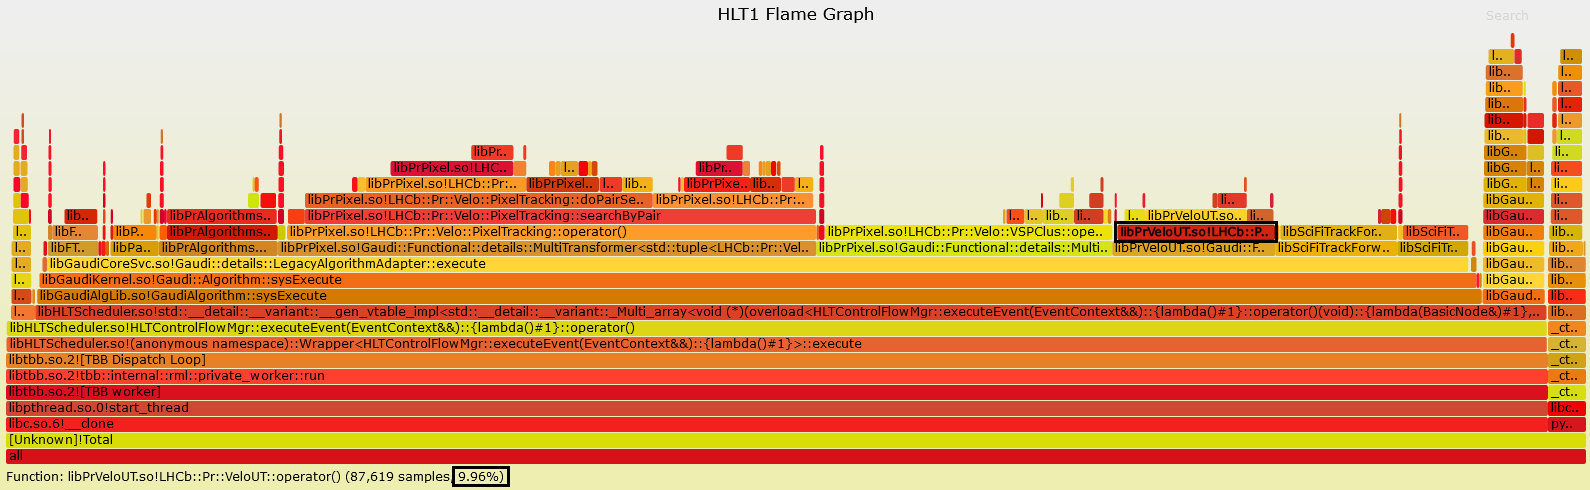
\includegraphics[width=\textwidth]{velout_flamegraph}
	\end{center}
	\caption[CPU time share of the VELO-UT algorithm]{The flame-graph shows the CPU time share of the algorithms. Share is proportional to the width of the bar that represents the particular algorithm. The entire width of the graph corresponds to 100\%, while the VELO-UT (highlighted with the black rectangle) reads 9.96\%.}
	\label{fig_velout_flamegraph}
\end{figure}


\subsection{Geometry of the UT detector}

\begin{figure}[H]
	\begin{center}
		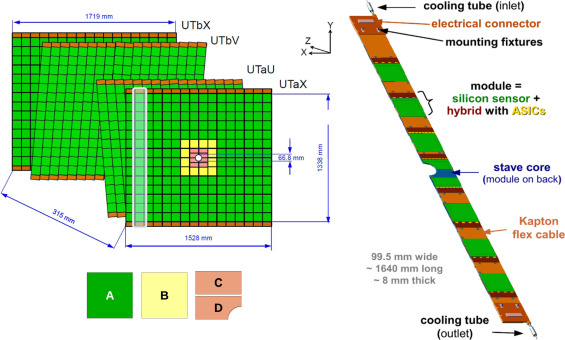
\includegraphics[width=0.9\textwidth]{detector_ut_geometry}
	\end{center}
	\caption[UT detector hardware blueprint]{Illustration of the key elements of the UT hardware. \cite{tracker_tdr}}
	\label{fig_ut_geometry}
\end{figure}

Figure \ref{fig_ut_geometry} shows the rectangular panels of the UT as looking down the detector from the VELO. The UT detector consists of four panels, their placement in the entire detector can be seen on figure \ref{fig_lhcb_geometry}. Each of the four panels is made up of 10 cm by 10 cm sensors. Though both the front two and rear two panels contain 14 rows of sensors, the rear panels are wider. The middle two panels have their sensors tilted by +5 and -5 degrees, which helps to mitigate the poor vertical resolution resulting from using silicon strips instead of pixel detectors. Each sensor contains silicon strips that run the full length of 10 cm of the sensor. There are 512 strips next to each other on every sensor. The exceptions are the sensor near the center of the panels, since the ones marked in yellow contain 1024 strips, and the ones marked in red contain 1024 half-length strips. The higher density area in the middle is required to deal with increased luminosity in the axis of the beam pipe. For each collision event, the software receives a list of the silicon strips that were hit by a particle. The Technical Design Report for the LHCb tracker\cite{tracker_tdr} explains the geometry in more detail.


\subsection{Decoding of the raw data from the detector}

Each silicon strip has a unique numeric identifier. During a collision event, the electronics of the UT detector compile a list of identifiers of the strips that were hit by a particle, which the software receives in a heavily compressed format. With a description of the exact geometry of the detector, that is, the location and dimension of sensors and strips in the global 3D space, the software is able to represent the strips that were hit by a line segment in the 3D space instead of just an ID. The \code{UTHits} resulting from the  decoding process are gathered into a \code{HitHandler} structure, which groups the hits by which sensor they belong to. The VELO-UT algorithm consumes the \code{HitHandler} alongside the VELO tracks to produce \textit{upstream} tracks.


\subsection{The original VELO-UT algorithm}\label{sec_velout_desc}

The main idea of the VELO-UT algorithm is to consume the VELO tracks and the UT hits, and extend the VELO tracks with hits from the UT to create so called \textit{upstream} tracks. The algorithm handles each VELO track separately. The process for a single VELO tracks can be broken down into the following steps:

\begin{enumerate}
	\item Skip track if it's unsuitable
	\item Extrapolate VELO track to the UT detector
	\item Gather UT hits that are close to the extrapolated track
	\item Find 3 or 4 UT hits that align in a line (1 hit per panel, sometimes one panel is missing)
	\item Analyze the \textit{track candidates} that consist of the VELO track + 3-4 UT hits
	\item Select the best candidate (if any is good enough) to extend the VELO track
\end{enumerate}


\subsubsection{Filtering tracks}

Any kind of tracks can be fed into the algorithm from the VELO tracking. Some tracks point to the wrong direction, away from the UT, other tracks go very close to the beamline and hit the central hole in the UT's panels, and some tracks may also simply miss the UT's panels as they go too much to the sides. These tracks are not worth trying to extend because there will be no solution, so they are dropped.


\subsubsection{Extrapolating tracks}

Tracks from the VELO are described by the \textit{state} of the particle. The state is a tuple of x,y and z coordinates, and the slopes tx=dx/dz and ty=dy/dz. In other words, the particle has a position [x,y,z] and has a velocity vector in the direction [tx,ty,1]. The usual coordinate system (see \ref{sec_coordinate_system}) is used for the states as well. To gather UT hits, one has to know where a track crosses a particular panel of the UT, which can be calculated by extrapolating the x,y,z position of the state to the z position of the panel along the line given by the slopes.


\subsubsection{Gathering UT hits}

Once the state is extrapolated, one can collect hits of the panel that are close to the x and y position of the extrapolated state. The implementation of the algorithm first collects the list of the 10 by 10 centimeter sensors that fall close enough. In case the track passes through the middle of one sensor, only one sensor will be tagged, however if the track hits the corner between four sensors, all the four may be tagged. Afterwards, the algorithm iterates through all the hits that belong to the tagged sensors, and checks for each hit if they are within tolerance to the extrapolated state. This, including the extrapolation, is repeated for all four panels, thus the final result is a set of close-by hits for each of the four panels for each track.


\subsubsection{Finding aligned hits}

There are on average 2-3 hits returned for each panel. Among these hits, the algorithm tries to find 3 or 4 hits that form a fairly straight line. These are called track candidates, and since there may be multiple sets of hits that form a straight line, the algorithm must decide on which is the best candidate.


\subsubsection{Analyzing candidates}

Each candidate that belongs to a track goes through a fitting stage. This is much like curve fitting or linear regression, the algorithm finds a mathematically optimal set of parameters that best describe the path of the particle that have created the UT hits of the candidate. 


\subsubsection{Selecting the best candidate}

The error of the fitting of a candidate can be calculated by determining how far the parameterized path of the particle lies from the position of the UT hits it was fitted from. If any of the candidates have a sufficiently low error, the one with the lowest is picked to form the newly created upstream track.


\subsection{Analysis of the original VELO-UT algorithm}

\subsubsection{Hotspots}

\begin{figure}[H]
	\begin{center}
		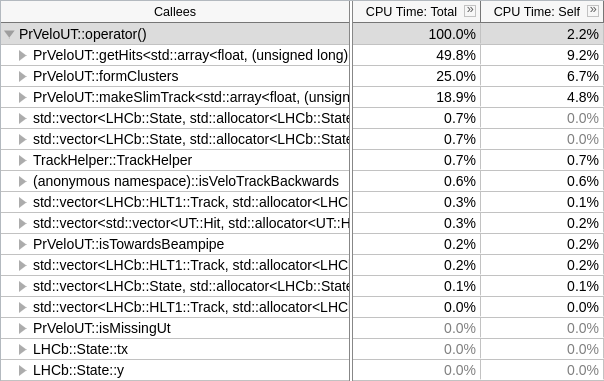
\includegraphics[width=0.7\textwidth]{velout_hotspots_orig}
	\end{center}
	\caption[CPU hotspots of the unoptimized VELO-UT algorithm]{Results of hotspots profiling with Intel VTune.}
	\label{fig_velout_hotspots_orig}
\end{figure}

As we can see, the VELO-UT algorithm spends most of its time gathering the UT hits that could potentially belong to a VELO tracks. The second largest portion is \textit{formClusters} which performs the search for aligned UT hits and also does a preliminary fit to determine the best candidate. The third largest unit is the creation of the output (the \textit{upstream} tracks) which performs a higher quality final fit and does some analysis to remove potentially undesirable tracks.

In light of this, the primary target for improvement is the largest chunk: gathering the hits, however, the other hotspots are also of significant interest.


\subsubsection{Gathering hits}

Examining the code of the hit gathering function (code listing \ref{lst_velout_gatherhits_original}), we can see that the main idea is to loop over the four planes, extrapolate the track to the plane, and collect the hits for each plane.

The first step in locating the close-by UT hits happens by finding the sectors (that is, the 10-by-10 centimeter sensors) that are adjacent to the point where the extrapolated track hits the current panel. The \code{findSectors} function performs this step via a rather complex logic (which is not shown here).

Given the sectors of interest, a loop goes over the sectors and queries the list of hits that belong to that sector from the \code{HitHandler}. The \code{HitHandler} already has the UT hits grouped by sectors, so this operation is rather simple.

Finally, the \code{findHits} function loops over the hits that belong to one sector, and keeps the hits that are truly close to the extrapolated track. Truly close here means that the fiber, when fattened into a cylinder, intersects with the line of the extrapolated track. (In reality, a simpler x and y tolerance is used instead of the heavy ray-cylinder intersection calculations.)

The final result is an \code{std::array} which contains four \code{std::vector}s of hits.

\vspace{1pc}

Looking at the code, we can spot several issues:
\begin{enumerate}
	\item Getting the list of nearby sectors is complicated: the sectors do not form a regular grid because of the smaller ones in the middle, which needs to be handled when doing lookups by x,y coordinates.
	\item Found sectors may be duplicated, as indicated by line 319-320, which is handled by special cases again and additional logic.
	\item Early exit conditions to cut computation time on lines 299, 302 and 320.
	\item Sectors are too coarse resolution for space partitioning, 10 centimeter's worth of fibers have to be checked for hits when the window is 2 centimeters at most.
\end{enumerate}

Issues \#1, \#2 and \#4 indicate that more work is done than absolutely necessary, while branching caused \#2 and \#3 may directly affect the performance on modern superscalar CPUs with deep pipelining. The idea with early exit conditions is to skip computation that will prove useless, however if the CPU misses the branch prediction, it has to flush its entire pipeline and restart the other branch. It is often a better approach to vectorize the branchless code and do the unnecessary calculations as well, then filter only the final results (with similarly vectorized code). Overall, the code is not vectorized at all, and does not have data-structures that would allow for vectorization.

In addition to performance problems, as the code is not clearly structured, optimization opportunities are easy to miss and hard to exploit, for humans and compilers alike.

\begin{figure}[H]
	\centering
	\begin{subfigure}{.5\textwidth}
		\centering
		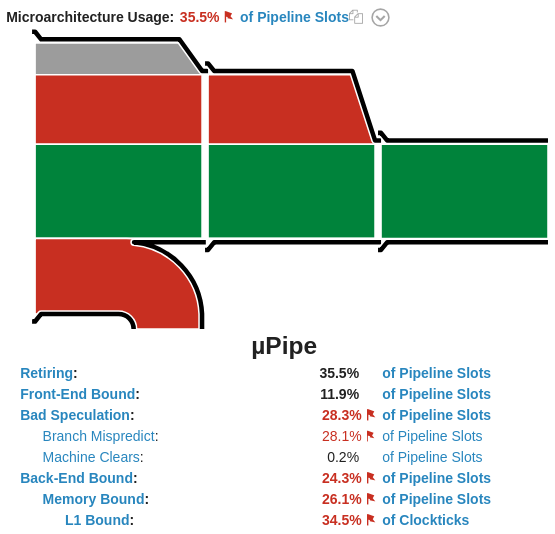
\includegraphics[width=\linewidth]{velout_gatherhits_orig_uarch}
		\caption{Microarchitecture usage of gathering\\ hits in the original code}
		\label{fig_velout_branch_example_sub1}
	\end{subfigure}%
	\begin{subfigure}{.5\textwidth}
		\centering
		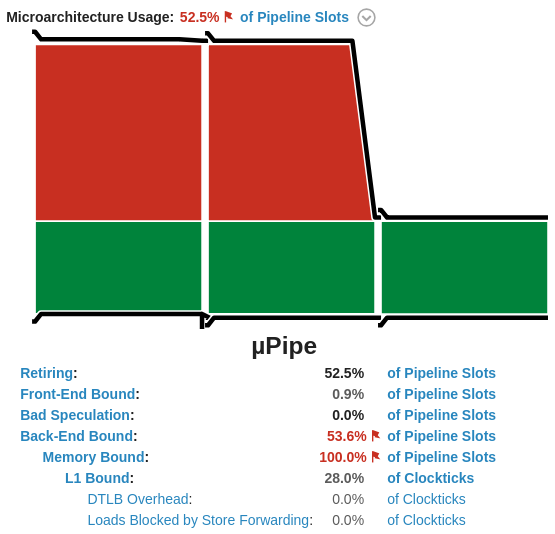
\includegraphics[width=\linewidth]{velout_gatherhits_new_uarch}
		\caption{Microarchitecture usage of gathering\\ hits in the refurbished code}
		\label{fig_velout_branch_example_sub2}
	\end{subfigure}
	\caption{Microarchitecture usage characteristics before and after rewriting the UT code.}
	\label{fig_velout_branch_example}
\end{figure}

Figure \ref{fig_velout_branch_example} shows the overall CPU microarchitecture usage of the current hit gathering compared to the new one. The low percentage of retiring instructions (35.5\%) is alarming. Additionally, 28.1\% of instructions are dropped due to branch mispredictions, which confirms the source code analysis that flow control is excessively complex and shows how much it impacts performance.
\newpage
\lstinputlisting[
	caption=Hit gathering for the original VELO-UT,
	label=lst_velout_gatherhits_original,
	language=C++,
	firstline=277,
	lastline=332,
	firstnumber=277]
	{source_code/PrVeloUT.cpp}
\newpage

\subsubsection{Finding aligned hits}

The largest part of the hit finding function is in fact the fitting of the aligning track candidates. Fitting is a simple, linear stream of mathematical operation with no branching, thus makes a perfect candidate for vectorization. However, vectorization cannot be exploited unless it is completely separated from the alignment search.

\begin{figure}[H]
	\begin{center}
		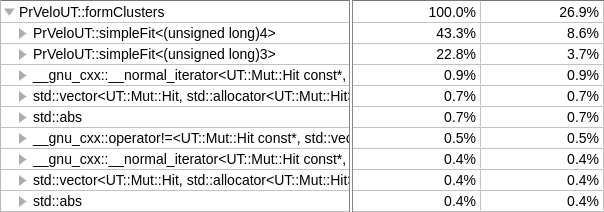
\includegraphics[width=0.7\textwidth]{velout_hotspots_orig_formclusters}
	\end{center}
	\caption[CPU hotspots of the VELO-UT aligned hit search]{The breakdown of the aligned hit searching. The two \code{simpleFit} calls account for the fitting, while the remaining ~30\% is the alignment search.}
	\label{fig_velout_hotspots_orig_formclusters}
\end{figure}


\subsubsection{Creating the final track}

The data format of the final track is not optimal. A track is represented by its own class, which dynamically allocates memory for the small number of hits and other objects it has. Transforming the track into a structure of arrays format is something to consider, which means for example that all the hits for all the track would reside in a large array, and the individual tracks would be indices into that array.
Additionally, as part of the creation of the track, a final, more accurate fit is performed. This is also a prime candidate for vectorization when separated from the rest of the code, and may also be merged with the preliminary fit to provide simpler and faster code, and potentially better results.


\subsubsection{General code design}

The code violates several coding best practices, which is not strictly an optimization problem, but is still an important concern as it is hard to find optimization opportunities in code that is hard to reason about. The most severe breaches are the single responsibility and dependency inversion principles. An example for the former is \href{https://gitlab.cern.ch/lhcb/Rec/blob/1b7edc5aea96f2225601238b3f64e478e41b6c70/Pr/PrVeloUT/src/PrVeloUT.cpp#L337}{\code{formClusters}}, which not only finds aligned hits but also parametrically fits them, an example for the latter is \href{https://gitlab.cern.ch/lhcb/Rec/blob/1b7edc5aea96f2225601238b3f64e478e41b6c70/Pr/PrVeloUT/src/PrVeloUT.h#L191}{\code{simpleFit}}, which modifies the flow control of its caller (formClusters) via modification of in-out (quasi-global) parameters. When the problems are alleviated, the search for aligned hits and the fitting can be done completely separately, which provides a massive gain thanks to the perfect vectorization of the fitting process.


\subsection{Design of the improved algorithm}

\subsubsection{Uniform grid space partitioning}\label{sec_velout_space_partitioning}

For the logic part, I left the algorithm as it was as I could not find better alternatives (see \ref{sec_velout_alternative}), however I redesigned space partitioning from scratch.
\vspace{1pc}

Space partitioning, most prominent in 3D graphics and physics simulations, is a technique to accelerate computations that are done on a large number of objects contained in a 3D space. Frequently, there are only significant interactions between nearby objects, so computations for the interactions of far away objects can be neglected. To be able to quickly list objects nearby to a 3D coordinate, I used the simplest space partitioning scheme: uniform grid. This method slices the 2D or 3D space by a uniform grid, and keeps a list of objects for each grid cell that fall into the cell. This way, to find objects near to a specific point, one only has to calculate the grid cell the point falls in (a few divisions) and read the list of that cell. (In some cases, the nearest four cells can be used not to miss any objects in case the specified point lies close to a grid line.) The logic of the grid-based lookup is vastly simpler than the sector-based lookup.
\vspace{1pc}

Since there are 14  rows of sensors on every plane of the UT detector, I used a grid with 14 rows, carefully aligned to the geometrical position of the sensor rows. This ensures that a fiber falls entirely within its grid cell. For the half-height sensors in the middle, two sensors fall into the same grid cell. There are no such limits for the horizontal resolution of the grid cells, so the cell width can be set arbitrarily. As the search region in the order of a few centimeters, I chose to have 64 cells on the horizontal axis, resulting in a cell width of roughly 3 cm. The third axis - in the direction of the beamline - is divided so that each four panel of the UT falls into its own grid cell. To sum up, the grid is 64 x 14 x 4 cells (see figure \ref{fig_velout_space_partitioning}).

The binning (assignment of cell) of hits is done by taking the middle point of the fiber, and using a division on all three axes to determine the integer coordinates of the corresponding cell.

Similarly, lookup of hits nearby to a point involves first a similar division to acquire the corresponding cell, then the hits assigned to that cell can be iterated over. One caveat, however, is that the middle two layers are tilted, so some tilted fibers cross multiple cells. In this case, we would like to have them show up when we query either of the cells. Instead of duplicating hits, I chose to simply sample the nearest two cells instead of just one (see figure \ref{fig_velout_space_partitioning}). With the cell size of 3 centimeters, it is unlikely to miss a hit in such way. The same issues persists in the vertical direction as well when the sampled point falls very close to a grid line. This is exacerbated by the small displacement on the Z axis that the sensors have by design of the hardware, and manufacturing errors also add to the problem. However, by design, there is a small overlap between two adjacent sensors, both on the vertical and horizontal axes. This means that a track hitting a grid line is likely to excite two fibers at the same time. The idea is that even when avoiding double-sampling on the vertical axis, at least one of those fibers will still be registered in the subject cells.

\begin{figure}[H]
	\begin{center}
		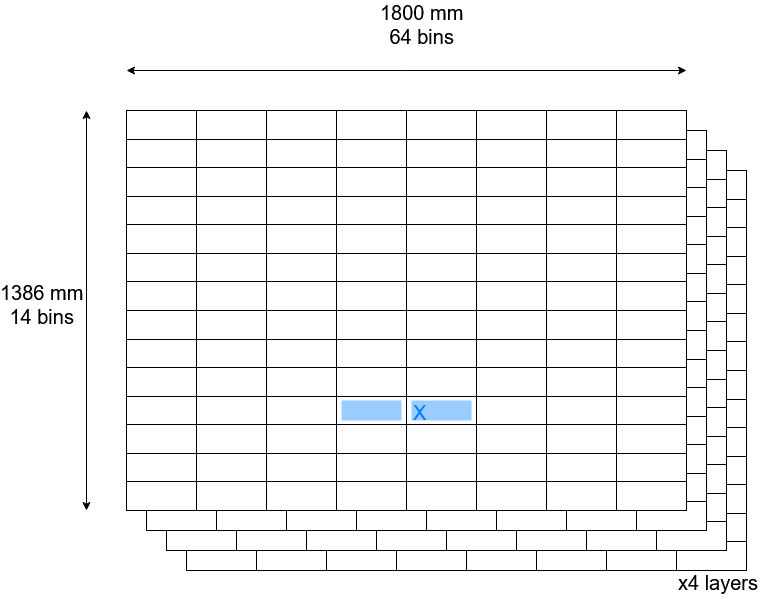
\includegraphics[width=0.85\textwidth]{velout_space_partitioning}
	\end{center}
	\caption[Uniform grid space partitioning]{Illustration of the bins of the space partitioning scheme. (Note that X only shows 8 cells as opposed to the actual 64 in order to make the image clearer.) As an example, the blue X marks the point where a particle's track crossed the detector, and the two adjacent grid cells highlighted in blue are searched for nearby fiber hits.}
	\label{fig_velout_space_partitioning}
\end{figure}


\subsubsection{Data structures and steps}

\begin{figure}[H]
	\begin{center}
		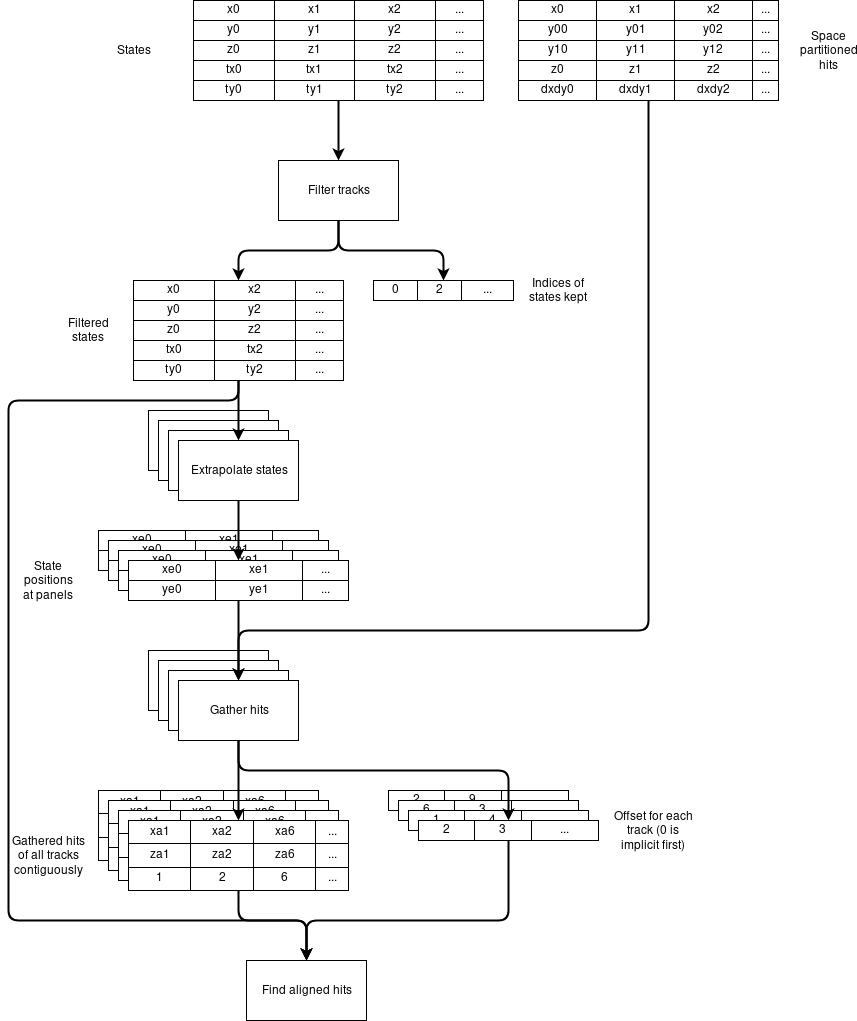
\includegraphics[width=0.85\textwidth]{velout_opt_datastruct_flow_p1}
	\end{center}
	\caption{Data structures and process diagram of the new VELO-UT algorithm. (Part 1)}
	\label{fig_velout_opt_datastruct_flow_p1}
\end{figure}

\begin{figure}[H]
	\begin{center}
		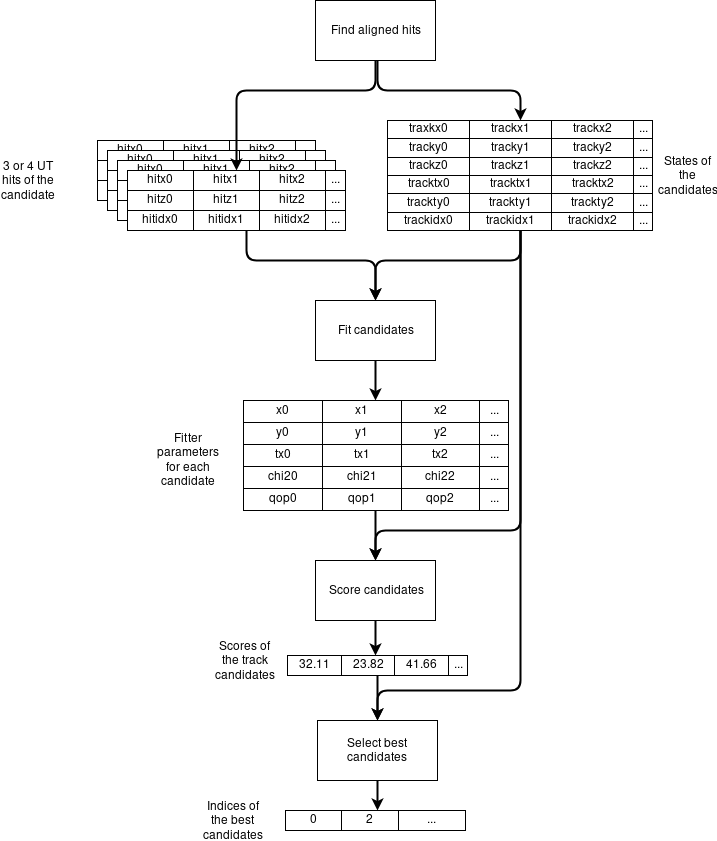
\includegraphics[width=0.7\textwidth]{velout_opt_datastruct_flow_p2}
	\end{center}
	\caption{Data structures and process diagram of the new VELO-UT algorithm. (Part 2)}
	\label{fig_velout_opt_datastruct_flow_p2}
\end{figure}

\paragraph{Layout of data} \mbox{}\vspace{0.4pc}

Figures \ref{fig_velout_opt_datastruct_flow_p1} and \ref{fig_velout_opt_datastruct_flow_p2} show the main steps of the algorithm as well as the exact data structures passed around. The data structures are structures of arrays (SOA), which are represented by tables on the drawing. Each row corresponds to a certain variable, while the columns usually represent variables that belong to a certain track. In memory, rows are stored in a contiguous block separate from other rows.

The SOA layout serves three purposes:
\begin{itemize}
	\item when reading a row, contiguous memory accesses are dispatched to the CPU, which makes it easy for the prefetcher to get data in the fast caches even before its used,
	\item for vectorization, operations can be done on multiple columns at the same time without de-interleaving the data,
	\item reading only a subset of the rows (i.e. only x and y but not z) incurs no waste unlike an AOS layout, where z would be loaded as it's in the same cache line.
\end{itemize}

Although SOA layouts generally make code harder to read and write, they are crucial to maximally exploit modern CPU architectures in performance critical applications.

\paragraph{Data} \mbox{}\vspace{0.4pc}

\begin{enumerate}
	\item States: a structure of five arrays that contain an x, y and z the track passes through, and the track's direction vector tx,ty,1.
	\item Space partitioned hits: as described in \ref{sec_velout_space_partitioning}, the hits are space partitioned by panels by rows by bins. All the hits reside in a large structure of arrays. The array begins with the hits of panel 0, row 0 and bin 0, then continue with bin 1, bin 2 and so on.
	\item Filtered states: a subset of States.
	\item Extrapolated states: one for each filtered state, only the x and y positions of the state are stored as z is known and tx and ty are the same as in the filtered states.
	\item Gathered hits: a partitioned array of hits that begins with the hits that belong to extrapolated state 0, then the hits for extrapolated state 1 follow and so on. Only the x and z of the fiber's closest point to the track is stored in addition to the index of the original hit in the space partitioned hit array. There are four such arrays, one for each panel.
	\item Offset for each track: for each extrapolated state it tells the index of the last hit inside the gathered hits array.
	\item 3-4 UT hits and states of the candidates: for each extrapolated state, zero or more candidates are constructed. The arrays store various parameters, included the four hits the make the candidate and the index of the extrapolated state the candidate belongs to. Thanks to the index, there is no need for an explicit array that tells the offsets into this array for each extrapolated state.
	\item Fitter parameters: contains a set of parameters one-to-one correspondence with the candidates.
	\item Scores: a simple real number for each track candidate.
	\item Indices of best candidates: an array with as many elements as unique indices to extrapolated states in the array of candidates. Contains indices to the array of candidates that refer to the best candidate of the same extrapolated track.
\end{enumerate}

\paragraph{Steps} \mbox{}\vspace{0.4pc}

The steps illustrated on figures \ref{fig_velout_opt_datastruct_flow_p1} and \ref{fig_velout_opt_datastruct_flow_p2} are very much the same as described in \ref{sec_velout_desc}. However, the crucial difference is that in case of the optimized version, all these steps handle all tracks at once instead of being called once for every track. This is what essentially gives opportunity for vectorization.

\begin{enumerate}
	\item Filter states: takes an array of states and outputs the array of states that pass through the UT detector.
	\item Extrapolate states: takes the filtered states and extrapolates them to a specified z coordinate, writing out the x and y of the extrapolated state. The extrapolation is called four times, producing one output array for each of the four UT panels.
	\item Gather hits: takes the extrapolated tracks and the partitioned array of hits and writes the hits that match with a state into the output array. Called once for each UT panel.
	\item Find aligned hits: takes the gathered hits and partitioning information, and compiles a list of track candidates for each track. A candidate is a set of 3 or 4 UT hits that align to form a line that is nearly colinear to the track. A track may have zero or multiple candidates.
	\item Fit candidates: estimates the path of the particle that produced the candidate's UT hits by parameters, taking as input the candidates and writing out said parameters.
	\item Scoring candidates: from the estimated parameters of the candidates, creates a score based on how well the parameters approximate the path determined by the hits. The better the fit, the higher the score.
	\item Select best candidates: for each track, find the candidate with the highest score and writes out an array of which the ith element contains the index of the best candidate for the ith track.
\end{enumerate}


\subsubsection{Vectorization of filtering}\label{sec_velout_filtering_vect}

The filtering algorithm takes a set of States that describe the VELO tracks, and decides which ones are possible to be be extended into a VELO-UT track. Thanks to the restructuring of the overall data structures by my colleagues, the VELO-UT algorithm now only receives so called \textit{forward tracks} (\ref{fig_lhcb_track_types}) that point towards the UT. Consequently, the filtering must only remove tracks that fall out of the acceptance of the UT, that is, miss all the panels of the UT and cannot produce any UT hits.

Rephrasing the specification in computing terms, for the vector of a states, a vector of booleans has to be produced where each boolean indicates weather to keep the corresponding state, and then the vector of states needs to be collapsed to a new vector that only contains accepted states. Using SIMD, on can easily take 8 elements (on AVX ISA) from the rows of the states, thus do calculations on 8 states at once to produce 8 booleans. It is possible to efficiently leverage Intel's AVX2 instruction set to do the pruning of the 8 items at a good performance\cite{lemire_simd_prune}. First, the items of the 8-vector are permuted in order to bring the selected elements to the front of the vector and move the unused items at the back. Second, an unaligned memory store operation writes the entire 8 vector to the output data structure at a specific offset. For the next write, the offset is increased by the popcount (number of the selected items), which means the next write will simply overwrite the unselected items of the current operation. (See figure \ref{fig_velout_opt_simd_filter}.)

\begin{figure}[H]
	\begin{center}
		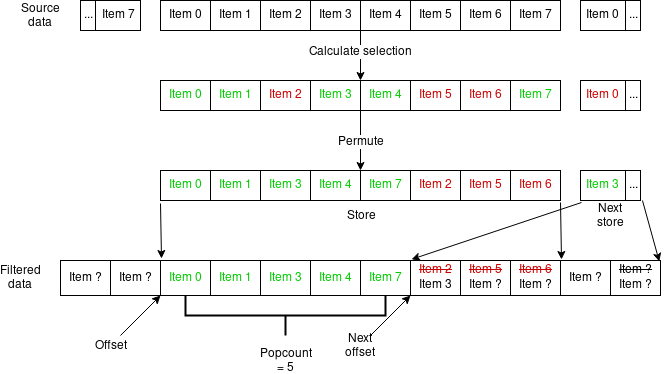
\includegraphics[width=0.85\textwidth]{velout_opt_simd_filter}
	\end{center}
	\caption{Visualization of the pruning step with 8-way SIMD}
	\label{fig_velout_opt_simd_filter}
\end{figure}

The large array of tracks are handled 8 at a time, producing the boolean mask, then doing the pruning, until the whole array is processed. The results of the filtering are stored in a format identical to the input states for consumption by later steps. Besides the states, an index array is also stored which contains the index of the selected states in the original table -- this is necessary bookkeeping to associate VELO track with their VELO-UT counterparts.


\subsubsection{Vectorization of extrapolation and fitting}\label{sec_velout_vectorize_extrap_fit}

The extrapolation and fitting code operates on a large array of tracks, it is pure computation with no branching, and the tracks are completely independent -- a perfect candidate for vectorization.

Extrapolation consumes full states that contain the position as well as the direction of the track, and writes out minimal states that contain only the x and y positions and the z of the UT panel we are extrapolating to. This makes sense, as tx and ty don't change, and the z is already known as it is tied to the panel, so the new x and y are enough. In case a subsequent process needs the remaining parameters, it can get it from the original array of states. This kind of split is an advantage of using SOA data layout. The implementation is a straight-forward loop that takes 8 tracks per iteration, does the extrapolation via vector registers, and writes out the 8 extrapolated tracks. The implementation of the fitter is in principle the same as the extrapolation, processing track candidates by batches of 8.


\subsubsection{Vectorization of gathering hits}\label{sec_velout_vectorize_gathering_hits}

To recap, the gathering of hits must iterate over each extrapolated state, obtain the panel, row and bin indices for the state, and query the range of hits in that bin from the space partitioner. Then, it has to iterate over the range of hits and select those that are close enough to the track, and write the selected hits contiguously into the output array.

The problem can be split into two parts:
\begin{enumerate}
	\item Getting panel, row and bin indices: as this step is the same, branchless pure computation (in theory) for each track, it can be perfectly vectorized.
	\item Iterating over the range of hits: vectorization simply over tracks is not possible, compiling a contiguous array of all hit candidates of all tracks seems expensive (although best for vectorization), so what's left is vectorizing over the range of hits but going scalar over tracks. The problem is that the number of hits in a bin is less than would be ideal for vector register of width 8, so a lower efficiency is expected.
\end{enumerate}


\paragraph{Getting bin indices} \mbox{}\vspace{0.4pc}

The x, y and z coordinates are given for each extrapolated state, the task is to figure out which grid cell they belong to. Given a uniformly partitioned axis, the bin index for a point can be calculated by evaluating
\begin{center}
	$t = (x_{state} - x_{min})/(x_{max} - x_{min})$\\
	$i =  \lfloor t \cdot N \rfloor$	
\end{center}
where $x_{min}$ and $x_{max}$ are the limits of the binned range and $N$ is the number of bins. The formula can be evaluated separately for the three axes, and it can be vectorized over 8 extrapolated states.

To obtain the offset and number of hits for a bin inside the partitioned array of UT hits, a lookup table that is indexed by the bin indices is available. The lookup can be either a scalar operation, or, as implemented, it can use the AVX gather instructions. For older CPUs, there is not much difference, gather instruction may be even slower, however recent Intel CPUs seem to perform better using gathers$^*$. One iteration thus returns two SIMD 8-vectors containing the offsets and the number of hits, which means it's completely vectorized.
\\
{
	\tiny
	\tab *: \url{https://stackoverflow.com/questions/24756534/in-what-situation-would-the-avx2-gather-instructions-be-faster-than-individually}
}

\paragraph{Filtering the range of hits} \mbox{}\vspace{0.4pc}

As the hits inside the range are not ordered by for example their x coordinates, all of them have to be examined. A vectorized filtering loop described in \ref{sec_velout_filtering_vect} is employed to select nearby hits from the range. Unfortunately, the average number of hits in a bin are in the order of 5 to 15 (depending on grid resolution), so using a SIMD register width of 8 allows for only 1 or 2 iteration per loop, which is less than ideal.

Storage of these hits is similar to the method described in \ref{sec_velout_filtering_vect} with the difference that the output is one big array that contains the gathered hits for all tracks. Consequently, an array of offsets is is also output which tells where to find gathered hits for a track in the aggregate array.

\paragraph{Double bins}\mbox{}\vspace{0.4pc}

As described in \ref{sec_velout_space_partitioning}, not a single bin but instead two adjacent bins are used. This changes the step for getting the bin indices minimally. Two lookups are performed, one for the actual bin index and another for the next or previous bin index, depending on which one the sampled coordinate is closer. (Double sampling only applies to bins, not row or panel indices.) The range is then defined by the offset of the first bin and the sum of the sizes of both bins. The hit filtering is unaffected, as it still takes an offset and a size, not caring where those come from.


\subsubsection{Hit alignment search}

The hit alignment search proved to be impractical to vectorize. The search algorithm operates on the nearby his gathered for a track. First, a pair of hits from two different panels are selected, a line is drawn through them, and the remaining two panels are searched for the hits closest to the line. In addition to the pair, an extra hit is accepted if it is within a threshold to the line. In case 3 or 4 hits (including the pair itself) were found that fall on the line, the track candidate is written to the output.

One average, there are only 2 hits per track per panel, so vectorizing over one member of the pair, the other member of the pair, and the extra hits is not practical. Vectorizing over the tracks if not feasible either, as the number of hits in the four layers can be very different between the track, and branching would ruin the vectorization. Other attempts, such as producing all 3 or 4 hit combinations and then determining if they are on a line is also impractical, as the generation would either be scalar code or inefficient vectorized code.


\subsubsection{Custom memory allocation} \label{sec_velout_stack_alloc}

With the optimized version of the VELO-UT algorithm, up to 20\% of the computation time was spent with memory allocation. The cost of memory allocation in an application depends most on the number of allocations, not the size of the allocations. Large allocations are much cheaper per byte allocated, so it is worth allocating an array for all objects upfront instead of allocating each object individually. The optimized VELO-UT algorithm uses this technique, however, the SOA data layouts require the allocation of a separate array for each data member of the structure. This combined with the fact that the algorithm generally works on a small amount of data makes memory allocations a significant problem.

\vspace{1pc}

Two options seems straightforward to reduce the number of memory allocations: allocating one large block of memory for all the contents of the SOAs, or using a global memory pool instead of turning to the system memory allocator. The latter results in simpler code and make it possible to reuse existing code such as the \code{std::vector}. Additionally, the way I'm implementing SOA containers through code generation with template metaprogramming and \code{std::vector}s, extending my containers with custom allocators like the STL itself is more natural.

\vspace{1pc}

The idea is to have a fast memory pool that it initialized at the beginning of the algorithm and torn down at the end. All memory allocations for the steps in-between are served from the pool instead of the OS memory allocator. This is achieved by initializing all \code{std::vector}s with this memory pool.


\vspace{1pc}

The choice fell on a stack memory allocator which works by requesting a large chunk of memory upfront from the operating system. A variable which shows the \code{offset} from the beginning of the chunk is initialized to zero.

\begin{figure}[H]
	\begin{center}
		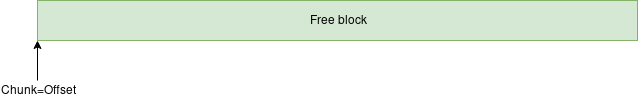
\includegraphics[width=\textwidth]{velout_stack_allocator_initial}
	\end{center}
	\caption{Initial state of the stack allocator.}
	\label{fig_velout_stack_allocator_initial}
\end{figure}

When memory is requested from the pool, a pointer at the current \code{offset} is returned to the caller. Internally, the \code{offset} is incremented by the size of the requested block, plus any padding if necessary.

\begin{figure}[H]
	\begin{center}
		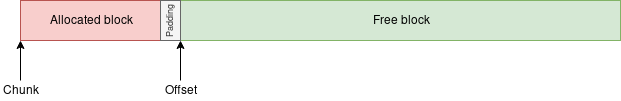
\includegraphics[width=\textwidth]{velout_stack_allocator_alloc1}
	\end{center}
	\caption{The allocator after the first allocation.}
	\label{fig_velout_stack_allocator_alloc1}
\end{figure}

Subsequent allocations are performed similarly.

\begin{figure}[H]
	\begin{center}
		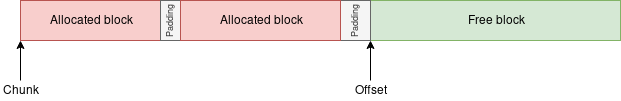
\includegraphics[width=\textwidth]{velout_stack_allocator_alloc2}
	\end{center}
	\caption{State of the allocator after a second allocation.}
	\label{fig_velout_stack_allocator_alloc2}
\end{figure}

Stack allocators are wasteful, because previously requested blocks are never individually deallocated and their memory reused, rather, all the memory is deallocated at once when the memory pool is destroyed. This, however, is not a problem, since the entire VELO-UT algorithm requires about half a megabyte from a stack allocator, which amounts to 20-30 megabytes of memory when running on 40-60 threads simultaneously. That is still negligible compared to more than 32 gigabytes of RAM which these machines are equipped with.

In case the allocator would run out of space, a new empty block is requested from the operating system. Even though this case is handled, the goal is to minimize the number of requests to the OS, so the initial block size is tuned so as to fit all data of the algorithm.

Stack allocators are extremely fast, as all it takes to allocate a new memory block is to return the offset pointer and increment the offset -- a couple of integer arithmetic instructions. Even though with the above extension an if statement handles the special case when it runs out of free space, the if rarely ever actually takes this path so the CPU should be hitting near perfect rates for branch prediction.


\subsection{Results}

\subsubsection{Overall performance}

I acquired the results by running the code on a Haswell\footnote{An Intel CPU architecture that supports the AVX2 and BMI CPU instruction sets my code needs} computer, looping over the same event for 100k iterations. The event of choice is a relatively busy event with many tracks. For the tests, the VELO-UT code was running alone, isolated from the rest of the reconstruction.

\begin{table}[H]
	\centering
	\begin{tabular}{c | c | c}
		& GCC 9.1 & Clang 8.0 \\
		\hline
		Original & 24157 ms & 21241 ms \\
		\hline
		Optimized & 9403 ms & 9744 ms \\
		\hline
		Opt. excl. SP & 6971 ms & 7589 ms
	\end{tabular}
	\caption{Execution time comparison of the VELO-UT algorithm after optimization.}
	\label{tbl_runtimes_local}
\end{table}
	
As the space partitioning is a new workload that wasn't present in the original algorithm, timings are shown with it included. The space partitioning can be, however, loosely considered as a replacement to the construction of the \code{HitHandler}, so timings with it excluded are also worth mentioning.

Overall, the optimized algorithm is 2.57x faster with GCC and 2.18x faster with Clang. When the space partitioning is excluded, the numbers are 3.46x and 2.80x, respectively. These numbers fall short to what one would expect by using 8-way SIMD instruction, however they better represent reality. As previously mentioned, a significant portion of the code remained scalar as it was difficult or practically impossible to vectorize and some of the vectorized code suffers from inefficiencies due to small amount of data in the vectorized loops. Additionally, the original non-vectorized code gets auto-vectorized by the compilers, which further shifts the balance. Overall, the speedup is still significant and worthwhile.

It is worth noting, however, that according to Amdahl's law, with about 75\% of the code vectorized with 8 parallel processors, the theoretical maximum gain is about 3x faster. Relating this to the measured numbers, the results are decent. There is an additional factor however, that the algorithm was slightly changed and uses the microarchitecture better regardless of the vectorization, which means the comparison with Amdahl's law is not perfect.

\begin{figure}[H]
	\begin{center}
		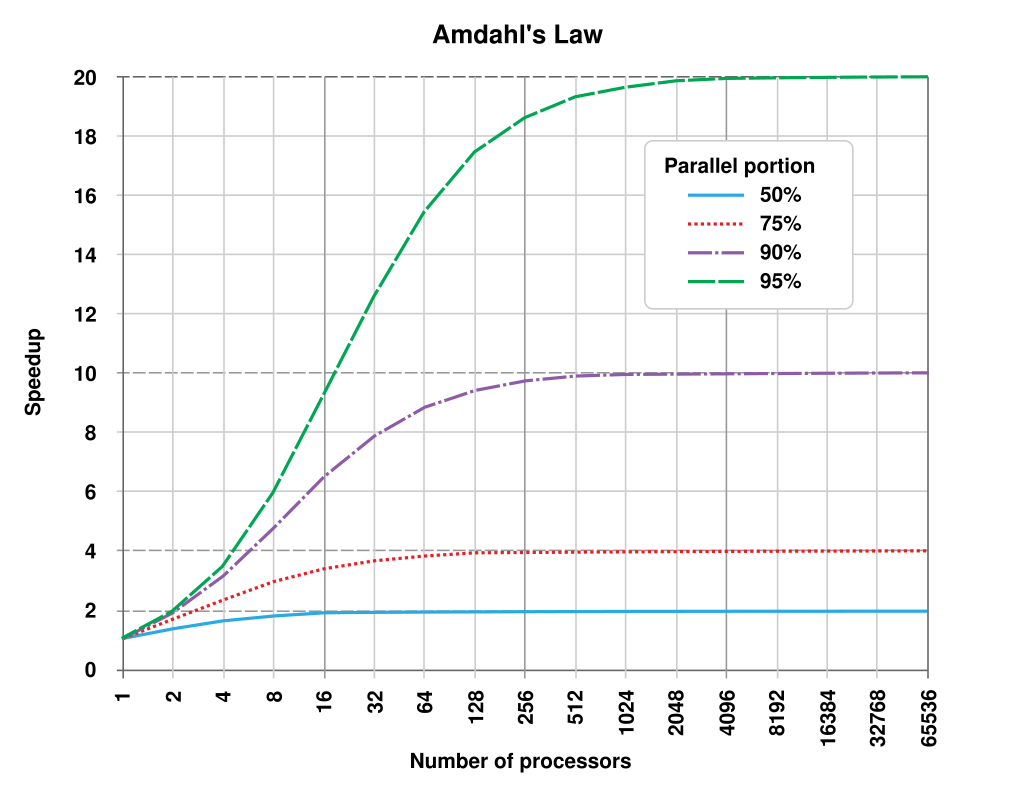
\includegraphics[width=\textwidth]{amdahls_law}
	\end{center}
	\caption[Amdahl's law applied to vectorization]{Amdahl's law shows how the performance gain is limited by the amount of remaining serial code.}
	\label{fig_amdahls_law}
\end{figure}


\subsubsection{Microarchitecture usage, bottlenecks}

\begin{figure}[H]
	\begin{center}
		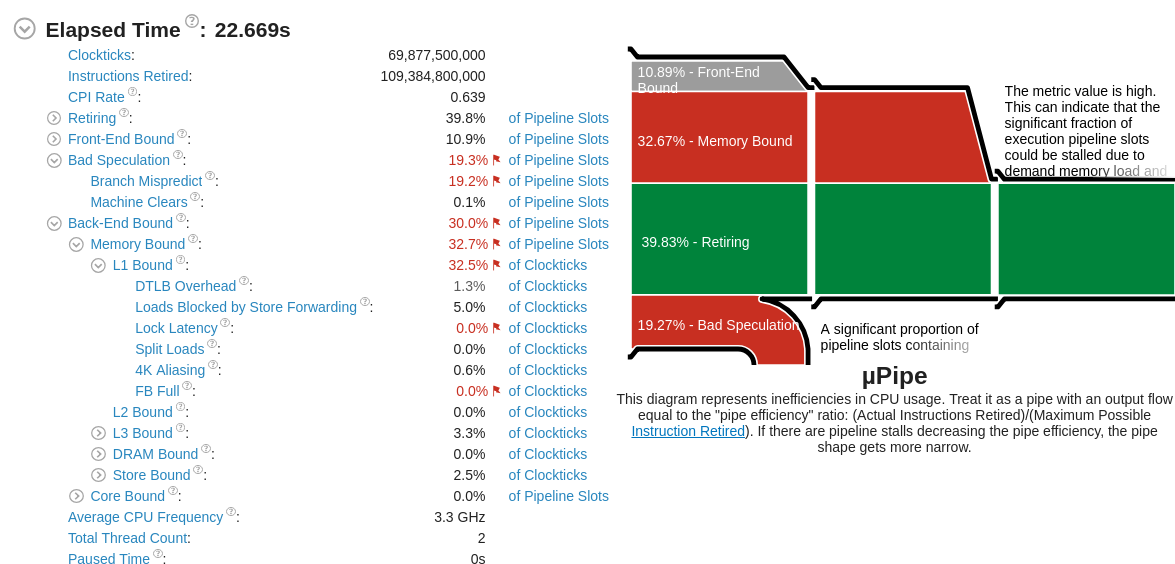
\includegraphics[width=\textwidth]{velout_uarch_overall_orig}
	\end{center}
	\caption{Microarchitecture usage of the original algorithm, results from Intel VTune.}
	\label{fig_velout_uarch_overall_orig}
\end{figure}

The two most significant problems with the original algorithm are being bound by memory and by bad speculation.

Understanding bad speculation is straightforward, if the CPU guesses to go on the \code{true} branch of an \code{if} statement and queues the upcoming instructions of that branch, but it happens that the \code{if} executes the \code{false} branch, all the queued instructions have to be cancelled.\cite{intel_vtune_docs} To alleviate this issue, one should remove branching altogether or, if not possible, make them more predictable.

As the profiler suggests, the code is mostly memory bound, more specifically, L1 cache bound. According to documentation from Intel, this metric shows up when the CPU is waiting for L1 load operations when the L1 cache was hit. This can happen, for example, when a load depends on an older store. To alleviate the problem, data dependencies can be rethought and the number of memory accesses per cycles spent with computation can be reduced.\cite{intel_vtune_docs}

\begin{figure}[H]
	\begin{center}
		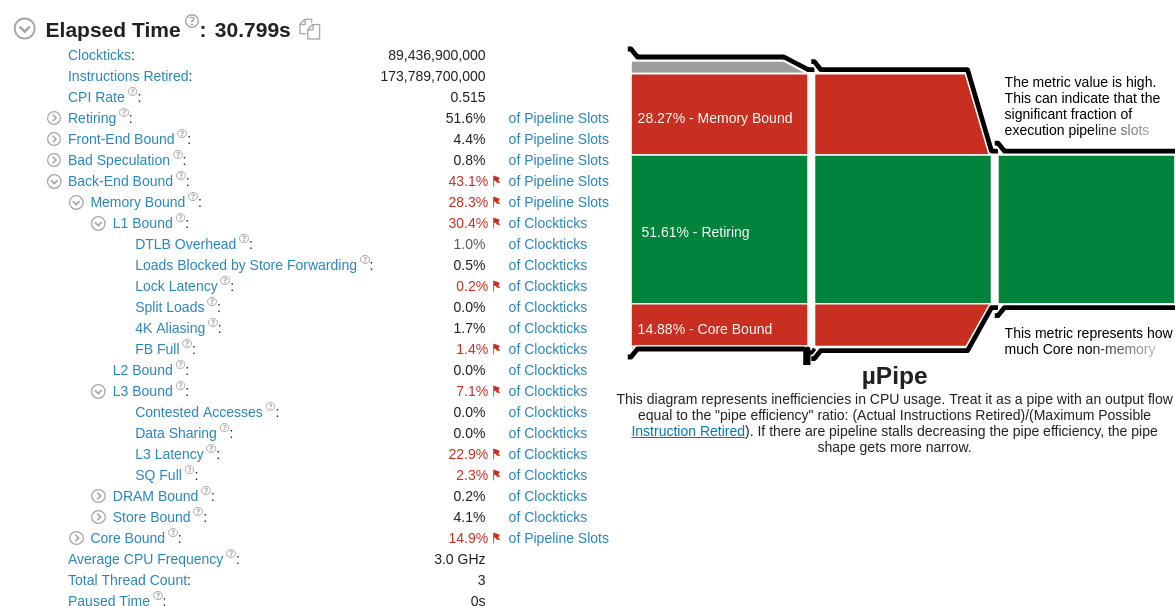
\includegraphics[width=\textwidth]{velout_uarch_overall_opt}
	\end{center}
	\caption{Microarchitecture usage of the optimized algorithm.}
	\label{fig_velout_uarch_overall_opt}
\end{figure}

Despite the optimized version being 2.5 times faster, the microarchitecture usage pattern shows some resemblance.

The most notable difference is the complete absence of bad speculation problems. I made a good effort to remove branching from the code so that computing passes can iterate over the entire datasets without conditional code execution. One trick to mitigate branching is in the filtering loops (\ref{sec_velout_filtering_vect} and \ref{sec_velout_vectorize_gathering_hits}) where masking and permuting of AVX registers is leveraged to emulate branching. Other tricks are, for example, the use of tiny branches which optimize out to CMOV instructions or the exploitation of boolean to integer conversion to obtain conditional numeric values by arithmetic instead of branching. The code for the fitting (\ref{sec_velout_vectorize_extrap_fit}) needs to handle track candidates with either 3 or 4 hits, but instead of branching, the unused hit in the 3-hit-case is simply masked out of the computations by using a weight of zero. This incurs a very little penalty, as the weight is needed for the algorithm regardless, and the elimination of branches allows for perfect vectorization.

\vspace{1pc}

Unfortunately, the algorithm is still the most heavily bound by memory accesses. VTune highlights L1 memory accesses similarly to the unoptimized version, but it does not indicate any specific issue in connection with L1. I examined the code of the gathering of the hits for data dependencies that could cause high L1 latencies, but it does not seem to show any. On the other hand, the code needs to read a lot of data, and does minimal calculation on it in comparison. Though this case is not mentioned in the documentation by Intel, a toy example of adding two small arrays that fit in L1 using vectorized instructions results in a heavily memory bound program according to VTune. Based on that, it simply seems like L1 is unable to serve the execution units of the CPU with enough data when the operations they do are too simple and fast. Since the algorithm already uses SOA data layouts and vector register loads to read only the most necessary data in the largest possible chunks, this is most likely a characteristic of the algorithm.

%\textcolor{red}{TODO: use roofline to check if code is ideal. See Omar Awile's talk in lhcb software tutorials.}
% I'm lazy plus I don't even have a machine that runs AVX2...

\vspace{1pc}

In place of branch prediction, VTune shows the algorithm is core bound. VTune indicates that this problems is to a lesser extent caused by overuse of the divider and to a larger extent by port utilization issues. The divider can be helped by using approximate divisions or factoring them out of loops, but the divisions were truly needed here. I tried to examine individual functions that are core bound due to port utilization, but I couldn't track down the source of the problem. The most prominent core bound function was \code{ScanExtraHits}, which contains a chain of dependent FP instructions, as indicated as a problem by the documentation\cite{intel_vtune_docs}. With GCC, which uses a fused multiply-add, the function is not core bound at all. Clang aggressively unrolls the loop even though it does two iterations on average, but does not use FMA, making the function core bound. When I forcefully disable loop unrolling, the function becomes even more core bound and the IPC dramatically decreases. It would need a significant amount of time to figure out and tune the function in isolation, which is not worth the effort.

\lstinputlisting[
	caption=Code of \code{ScanExtraHits}.,
	label=lst_velout_scanextrahits,
	language=C++,
	firstline=134,
	lastline=146,
	firstnumber=134]
	{source_code/PrVeloUtOpt.h}



\subsubsection{Effects of customized memory allocation}


\begin{figure}[H]
	\begin{center}
		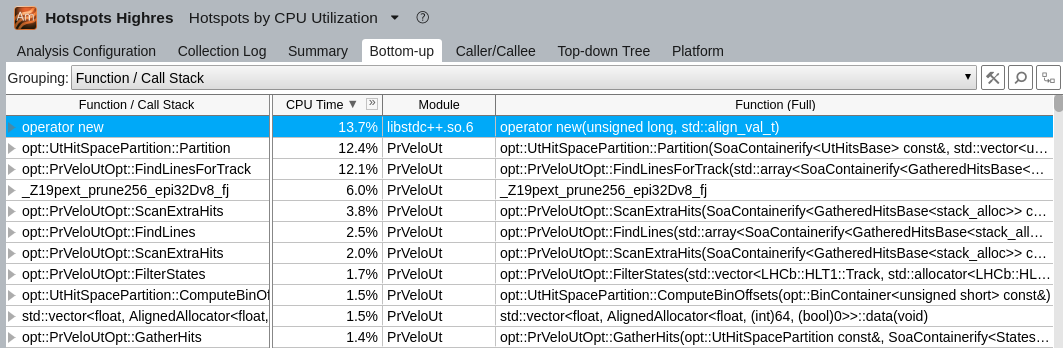
\includegraphics[width=\textwidth]{velout_without_alloc}
	\end{center}
	\caption[CPU hotspots \textit{without} custom allocator]{Hotspots profiling with VTune. Note the high amount of time spent in \code{operator new}.}
	\label{fig_velout_without_alloc}
\end{figure}


\begin{figure}[H]
	\begin{center}
		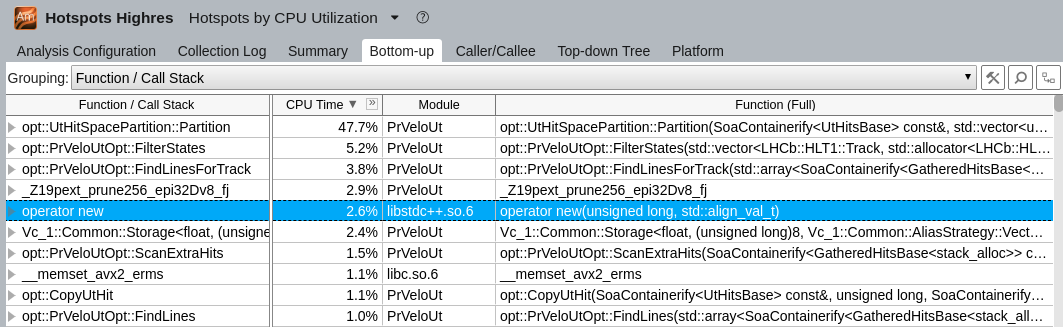
\includegraphics[width=\textwidth]{velout_with_alloc}
	\end{center}
	\caption[CPU hotspots \textit{with} custom allocator]{With the stack allocator, \code{operator new} has almost disappeared.}
	\label{fig_velout_with_alloc}
\end{figure}

Figure \ref{fig_velout_without_alloc} shows that without any special memory allocator, the program spends more than 13 percent in memory allocation. (Interestingly, the freeing of memory does not seem to take significant amount of computation.) However, thanks to the stack allocator, this can be reduced to less than 3 percent of the CPU time. The difference shown in the profiler manifests in the runtime as expected: 33.8 seconds with the default allocator compared to 29.1 seconds with the stack allocator, that is a gain of 14\%.


\subsection{Alternative VELO-UT algorithms}\label{sec_velout_alternative}

One of the main steps of the VELO-UT algorithm is to find hits in the UT that align to form a nearly straight line. Unfortunately, this step is serial code and it is very difficult (if at all possible) to vectorize, leading to slow performance. In order to produce code that is more easily vectorizable, I experimented with alternative methods to find a set of UT hits that align both with each other and a VELO track. While the methods did not work as expected, they are worth noting as they may work in different contexts.

\subsubsection{Parabola extrapolation of VELO tracks}

The first solution I tested was to extrapolate the straight VELO tracks through the UT. For the extrapolated section of the tracks, I used a parabola that smoothly aligns with the VELO track on one end and coincides with a hit from the last layer of the UT. As the next step, the single closest hit from the remaining 3 UT layers are assigned to the extrapolated track.

Since there may be multiple last-layer UT hits for each VELO track that fall within a certain window of the track's line, there will also be multiple extrapolated candidates per VELO track. To select the best candidate, the distance of the hits from the parabola are summed, and one candidate with the least error is selected.

The advantage of this method is that it eliminates the expensive and serial combinatorics involved in finding 4 aligned UT hits. Solely the last layer and the VELO tracks are used to seed extrapolated candidates, and once the data structures are built, calculating the parameters of the parabolas can be parallelized. The assignment of hits from the other layers is also straightforward as it can be parallelized over the hits within a window close to the parabola, and the problem is simply to pick the hit nearest.

\begin{figure}[H]
	\begin{center}
		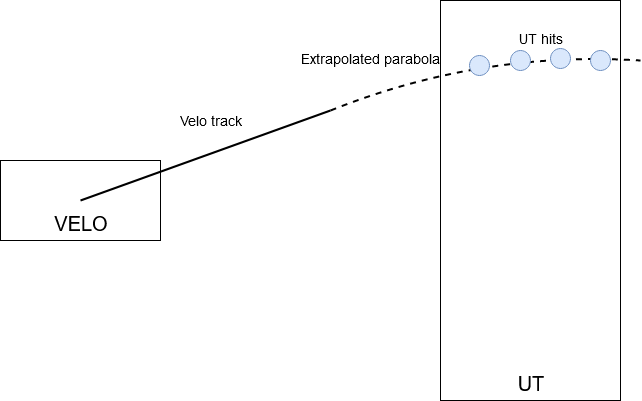
\includegraphics[width=.75\textwidth]{velout_parabola_fit}
	\end{center}
	\caption[Parabolic extension of VELO tracks]{Straight VELO tracks are extended by a parabola that align closely with UT hits.}
	\label{fig_velout_parabola_fit}
\end{figure}


Unfortunately, the algorithm did not produce good results form the physics perspective. In reality, the uncertainty in the VELO tracks' direction and position is too large so when extrapolated just linearly, the corresponding UT hits often lie on both sides of the line. In such a case, the parabola that is constrained to the VELO track's line on one end will show significant deviation from the real hits no matter its parameters. This means the extrapolation will pick up incorrect hits or will have errors too large to be taken as a valid solution.

\begin{figure}[H]
	\begin{center}
		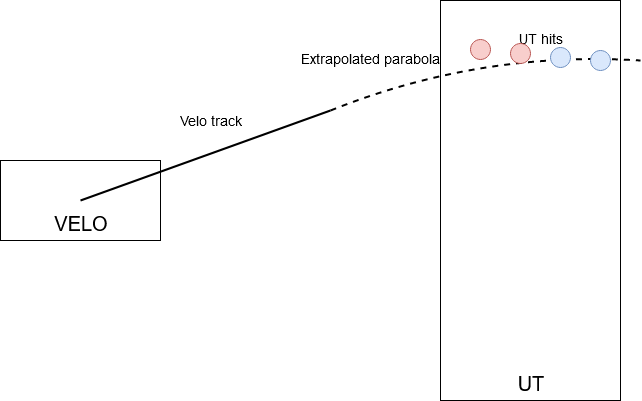
\includegraphics[width=.75\textwidth]{velout_parabola_misfit}
	\end{center}
	\caption[Misalignment of parabolic extension to UT hits]{How hits are often placed in reality. Note the hits marked in red, falling on the other side of the line of the VELO track, being largely misaligned with the parabola adjusted to the last-layer hit.}
	\label{fig_velout_parabola_misfit}
\end{figure}


\subsubsection{Hough-transform/gradient descent hybrid line finding}

The experiment with parabola extrapolation showed that the key is not the alignment of hits to the VELO track, but finding four hits that themselves align on a straight line very well. (The straight line is reasonable despite the slight bend of the particles due the magnetic field, especially as this is optimized for high-momentum particles that bend only a little.) The original line aligned hit finding extrapolates the VELO track as a straight lines and selects hits from each layer within a certain window of that line. Then each combination of four hits is tested if they lie on a straight line. While there are early exit conditions, such as not being able to find even a third aligned hit, this code is still poorly vectorizable and generally expensive because of the sheer number of combinations to be tested. The code also scales very poorly, as the more hits there are the exponentially more combinations it has to test.
\vspace{1pc}

A method that has a better time complexity to find lines in such a scenario is the Hough-transform\cite{wiki_hough_transform}. To construct the Hough space, one has to loop over all points, then increase all the pixels in the feature that correspond to a line through the point in subject. As this was not optimal for vectorization and low amount of calculation, I did it the other way around. For each point in the Hough space, I calculated how far the line represented by the Hough space point is from each of the image space and summed the distances up. Vectorizing over the Hough space is easy, and the task is now reduced to a minimum finding in the Hough space.

\begin{figure}[H]
	\centering
	\begin{subfigure}{.5\textwidth}
		\centering
		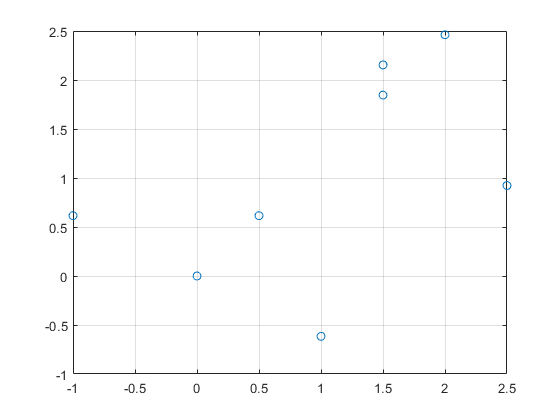
\includegraphics[width=\linewidth]{velout_hough_points}
		\caption{Points among which trying to find alignment}
		\label{fig_velout_hough_points}
	\end{subfigure}%
	\begin{subfigure}{.5\textwidth}
		\centering
		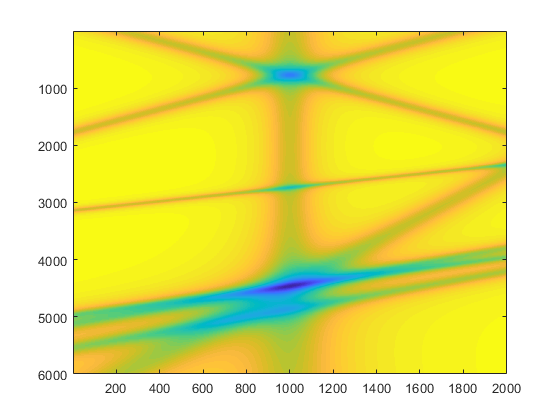
\includegraphics[width=\linewidth]{velout_hough_param_space}
		\caption{Resulting Hough space in high resolution}
		\label{fig_velout_hough_param_space}
	\end{subfigure}
	\caption[Point and the Hough-space of alternative line finding]{Among the points, we can spot the four on the diagonal that form a straight line. The parameters of this line correspond to the deep blue spot in the lower-middle part of the Hough-space. Less deep blues represent lines that go through 2 or 3 points.}
	\label{fig_velout_hough_method}
\end{figure}

To construct the Hough space, it was not enough to simply take the distance of the point and the line. Instead, I ran the distance through a function that converges to 1 at either ends and has a downwards bump in the middle with $f(0)$ being zero. This is the cause of the narrow greenish bands and the large yellow plateaus. Theoretically, one could run a gradient descent on the surface and find the absolute minimum with random search.
\vspace{1pc}

In the actual implementation, I did not do gradient descent on the high resolution image, but instead reduced the Hough space to be as small as 16 by 8 pixels. This was enough to specify the line with sufficient accuracy, and was small enough for the amount of calculation to be reasonable. Notice that in this case, there are three nested loops: 8 iterations over the width, 16 iterations over the height and iterations through all points/hits. The outer loop of 8 iterations corresponds to the SIMD width and is thus reduced to a single CPU instruction. In place of gradient descent, the 8-by-16 pixel area was brute-force searched for the smallest element using SIMD.
\vspace{1pc}

Despite reducing the amount of computation and vectorizing everything, the method did not work as its computation time was still too much. This is an interesting example where an $O(n!)$ algorithm (although with early exits) beats an $O(n)$ algorithm due to the large difference in constants.


%----------------------------------------------------------------------------
% === Conclusion ===
%----------------------------------------------------------------------------
\newpage
\section{Conclusion and future work}

This thesis touched three main topics:
\begin{itemize}
	\item Generic performance optimizations of the Kalman track fitter
	\item Modernizing the data model of the LHCb's first level trigger
	\item Leveraging vectorization to speed up the VELO-UT tracking
\end{itemize}
For the first task, streamlining the existing algorithm, removing unnecessary parts and simplifying the code resulted in a roughly two-fold speedup of the subject code.

The second task enabled the team to move towards the vectorization of the entire performance-critical code without losing performance gains in data layout conversions. Although significant speedup has already been achieved, the long term effects are even more favourable.

The third task made use of the new data model to vectorize an existing part of the code. The VELO-UT tracking has been sped up by about a factor of three.
\vspace{1pc}

This thesis work confirmed yet again how much code's performance can be improved with the right tools and coding practices. The work on the Kalman fitter has shown the importance of keeping the code clean and simple not only for readability but also for performance. The fastest code is the one that never runs. The new data model has highlighted the importance of understanding and utilizing modern CPU's features and avoiding their weaknesses. Writing cache-friendly and branchless code is essential. Finally, the latest instruction sets of modern CPUs allow hardware-based acceleration of specific tasks. SIMD instruction such as AVX and utility instructions such as BMI can improve performance significantly for scientific workloads.
\vspace{1pc}

Regarding the future, it is important to keep the code easy to change and to use programming abstractions that facilitate the migration to new CPU features as they come. As the majority of the software has not been vectorized yet, optimization efforts have to be extended to other areas of the code. The new data model, although functional, could definitely do with improvements to its interface to provide easier use and better safety.
As for the VELO-UT tracker, the physics performance is slightly lower than expected. It has to be investigated weather this is an issue, and if so, it needs to be fixed by slight modifications to the algorithm. Additionally, the aligned hit finding was not vectorized. Since that part takes up a significant portion of the CPU time, more performant methods could be implemented.



%----------------------------------------------------------------------------
% REFERENCES
%----------------------------------------------------------------------------
\newpage
\section{References}

\begin{thebibliography}{asd}
	\bibitem{cern_about} About CERN: \\
		\url{https://home.cern/about}
	\bibitem{cern_accel_complex} CERN's accelerator complex: \\
		\url{https://home.cern/about/accelerators}
	\bibitem{lhc_desc} About the Large Hadron Collider: \\
		\url{https://home.cern/topics/large-hadron-collider}
	\bibitem{lchb_desc} About the Large Hadron Collider beauty experiment: \\
		\url{https://home.cern/about/experiments/lhcb}
	\bibitem{lhc_lead_ions} Why collide lead ions: \\
		\url{http://alicematters.web.cern.ch/?q=FAQ-why-lead-ions}
	\bibitem{lhc_energy} Energy of the LHC: \\
		\url{https://home.cern/about/engineering/restarting-lhc-why-13-tev}
	\bibitem{lhc_bunch_collisions} LHC collisions: \\
		\url{https://lhc-machine-outreach.web.cern.ch/lhc-machine-outreach/collisions.htm}
	\bibitem{lhc_facts_and_figures} LHC facts and figures: \\
		\url{https://public-archive.web.cern.ch/en/LHC/Facts-en.html}
	\bibitem{kalman_filter_wiki} Explanation of Kalman filters: \\
		\url{https://en.wikipedia.org/wiki/Kalman_filter}
	\bibitem{kalman_filter_lhcb} Additional read on track fitting: \\
		\url{https://twiki.cern.ch/twiki/bin/view/LHCb/LHCbTrackFitting}
	\bibitem{tracker_tdr} Tracker (UT and FT) Technical Design Report: \\
		\url{https://cds.cern.ch/record/1647400?ln=en}
	\bibitem{god_class_wiki} God class anti-pattern: \\
		\url{https://en.wikipedia.org/wiki/God_object}
	\bibitem{lemire_simd_prune} Pruning with AVX2: \\
		\url{https://github.com/lemire/simdprune}
	\bibitem{intel_vtune_docs} Documentation of microarchitecture analysis by Intel: \\
		\url{https://software.intel.com/en-us/vtune-amplifier-help-core-bound}\\
		\url{https://software.intel.com/en-us/vtune-amplifier-help-l1-bound}\\
		\url{https://software.intel.com/en-us/vtune-amplifier-cookbook-top-down-microarchitecture-analysis-method}
	\bibitem{accelerator_image_src_1} Particle accelerators:\\
		\url{http://universe-review.ca/R15-20-accelerators01.htm}
	\bibitem{lhcb_coordinate_systems} LHCb Coordinate Systems:\\
		\url{https://edms.cern.ch/ui/file/372642/1/LHCb-coord-system.pdf}
	\bibitem{lb_event_display} LHCb Event Display:\\
		\url{https://lbevent.cern.ch/EventDisplay/index.html}
	\bibitem{tracker_image} L.B.A. Hommels: The LHCb outer tracker detector design and production\\
		\url{https://www.researchgate.net/publication/4154465_The_LHCb_outer_tracker_detector_design_and_production}
	\bibitem{lhcb_twiki} LHCB Wiki:\\
		\url{https://twiki.cern.ch/}
	\bibitem{cern_document_server} CERN Document Server, a collection of public documents of CERN:\\
		\url{cds.cern.ch}
	\bibitem{lhcb_tracking_strategies} LHCB Tracking Strategies:\\
		\url{https://twiki.cern.ch/twiki/bin/view/LHCb/LHCbTrackingStrategies}
	\bibitem{wiki_hough_transform} Hough-transform:\\
		\url{https://en.wikipedia.org/wiki/Hough_transform}
\end{thebibliography}


%----------------------------------------------------------------------------
% APPENDICES
%----------------------------------------------------------------------------

\newpage
\section{Appendices}

\appendix
\renewcommand{\thesubsection}{\Alph{subsection}}

\subsection{Intel VTune Amplifier XE}

The document includes many screenshots of Intel's VTune Amplifier XE. VTune is an advanced performance profiler that measures how long certain parts of the code take to execute. It operates by pausing the profiled process a few hundred or thousand times every second and noting down which line of code was executing at the moment of the pause. Over roughly a minute, VTune gathers enough samples so that they are largely statistically correct. In other words, if 90\% of the samples have been recorded for one line and 10\% of the samples for the other, the first line takes roughly 90\% of the CPU time while the latter takes 10\%.
\vspace{1pc}

In addition to line-based timing information, VTune also gathers complete stack traces, thus it can show the relative or absolute time certain functions have taken. VTune can visualize the relationship between functions in multiple ways.
\vspace{1pc}

Alongside the \textit{hotspots} profiling described above, VTune also can also analyze microarchitecture, threading and memory usage. Microarchitecture refers to how well the program utilizes the available functional units of the CPU, such as memory load/store, floating point unit, integer arithmetic and divider. Modern CPUs are able to perform multiple independent integer operations at the same time or overlap memory transfers with arithmetic. VTune attempts to highlight issues with pipelining or imbalanced load such as overstressed divider. VTune also helps analyze memory usage issues by providing information on main memory bandwidth, cache utilization and cache misses.
\vspace{1pc}

More information can be found on Intel's website: \url{https://software.intel.com/en-us/vtune}.

\subsection{LHCb track types}

Throughout the document, there are several \textit{track types} mentioned. In LHCb, tracks are classified based on which sub-detectors they interact with and which direction they have.
\vspace{1pc}

\noindent We differentiate the following track types:
\begin{itemize}
	\item Backwards track: exits the VELO the direction opposite to the other sub-detectors (not shown on figure \ref{fig_lhcb_track_types})
	\item VELO track: seen in the VELO, but does not interact with any other sub-detector
	\item Upstream track: interacts with the VELO and the UT
	\item Long track: interacts with all three of the VELO, UT and FT
	\item Downstream track: interacts with the UT and the FT (e.g. particle decay products from displaced secondary vertices)
	\item T track: only seen in the FT (decay products, similarly)
\end{itemize}

\begin{figure}[H]
	\begin{center}
		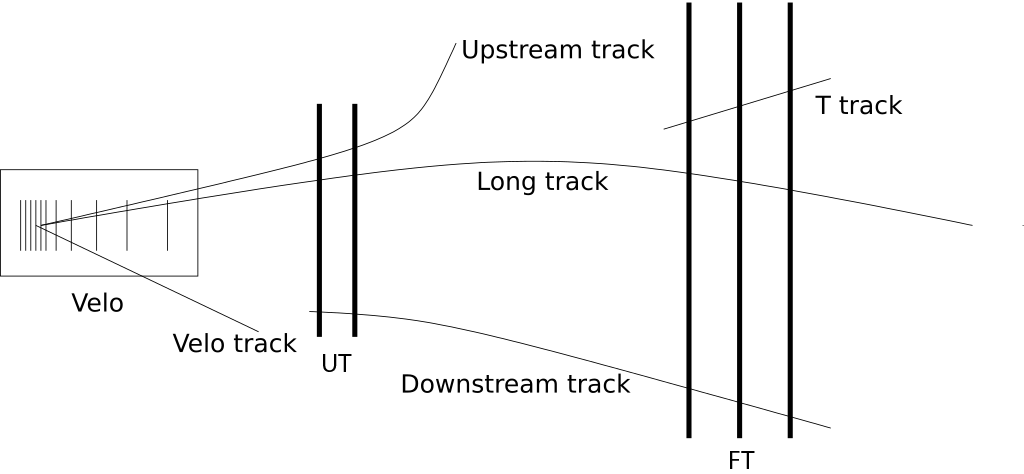
\includegraphics[width=\textwidth]{lhcb_track_types}
	\end{center}
	\caption[Types of tracks for LHCb]{Different track shown on the schematic of the LHCb detector.}
	\label{fig_lhcb_track_types}
\end{figure}


\subsection{LHCb software configurations}

The \textit{best physics} and \textit{best throughput} configurations are mentioned throughout the text. The LHCb trigger does not have one fixed implementation, rather, the parts it is made of can be combined and configured differently. Generally, performance (that is, throughput) can be traded for physics accuracy. There are several configurations tested at all times so that a good compromise between physics accuracy and throughput can be selected. The \textit{best physics} and \textit{best throughput} configurations are the two extremes.

The \textit{best physics} case includes complete processing of all data and an additional track fitting via the Kalman filter at the end. This, however, produces a generally low throughput. The \textit{best throughput} configuration introduces filtering early in the processing chain to keep only relevant tracks for further processing. Unfortunately, this filtering makes certain physics analyses impossible. Additionally, the final filtering may be reduced or omitted altogether for the \textit{best throughput} configuration.


%----------------------------------------------------------------------------
% END DOCUMENT
%----------------------------------------------------------------------------
\end{document}
